%==========================================================
% The template mechanism
%==========================================================
\chapter{The template mechanism}

\section{The master template}
%============================================================================
In this chapter, we start with showing the template mechanism by some examples that should be
modified by you. This way you should get used to the system and see that most templates can
easily be modified from the interface point of view. Thus, it is no problem if you don�t
understand all tags and functions that are used at the beginning, they will all be explained
later in this document in detail. Right at the beginning, you should try to find out how they
work and behave by working with them.

We will now create a first template set of a very simple kind. Our
first template set will not include any special sub templates and
will not define a special layout, but it should give a little
insight in the template mechanism.

The first example will show how to create a template set that
displays the string {\name Hello, world!}. A template set consists
of three templates. The frametemplate contains the design of the
Frame. The contenttemplate contains the elements and the bodies.
The master template only defines which frametemplate and which
contenttemplate should be used by the page. We will create a
template set of {\dir /content/templates/template1} (the master
template), {\dir /content/frametemplates/frametemplate1} and {\dir
/content/contenttemplates/contenttemplate1}. To create a template
you must first create a new text file in the project's {\dir
content/templates}. Go to the {\dir /content/templates} directory
in the Explorer view of the new project and start the wizard that
creates the new files by clicking on the icon with the magic wand.
Select {\name Text} for the type of the file from the New dialog
box (Figure~\ref{createOtherType}).

\begin{figure}[hbt]
\begin{center}
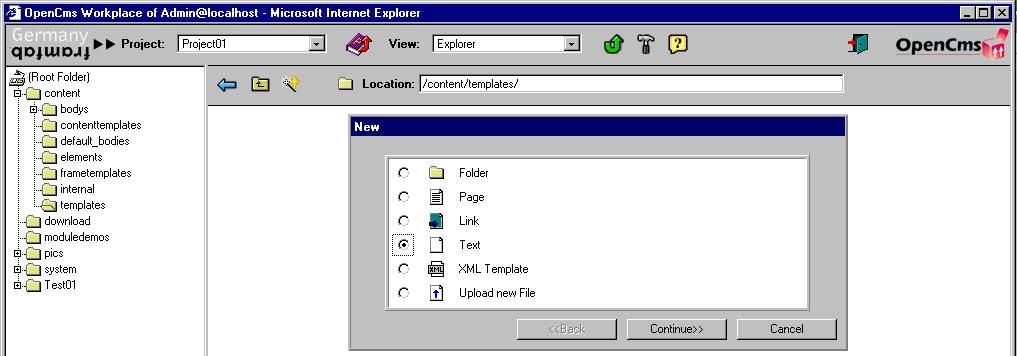
\includegraphics[width=\sgw]
                   {pics/templateMech/createOT}
\caption[Creation of a new template]
           {Select Text for the new file}
\label{createOtherType}
\end{center}
\end{figure}

Enter the name and title for the new template in the Create a new
File dialog box and click on {\name Finish} to end the creation of
the new text file (Figure~\ref{createOT2}).

\begin{figure}[t]

\begin{minipage}[b]{0.499\linewidth}
  \begin{center}
  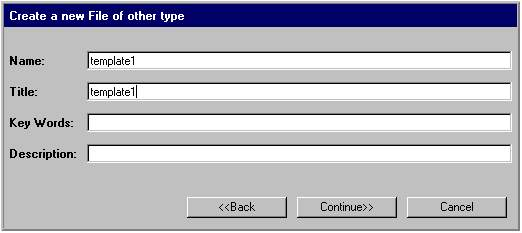
\includegraphics[clip,width=\sgw]
                   {pics/templateMech/createOT2}
 \end{center}
\end{minipage}
\hfill
\caption[Creation of a new template]
           {Enter name and title}
 \label{createOT2}

\end{figure}

\begin{figure}[hbt]
\begin{center}
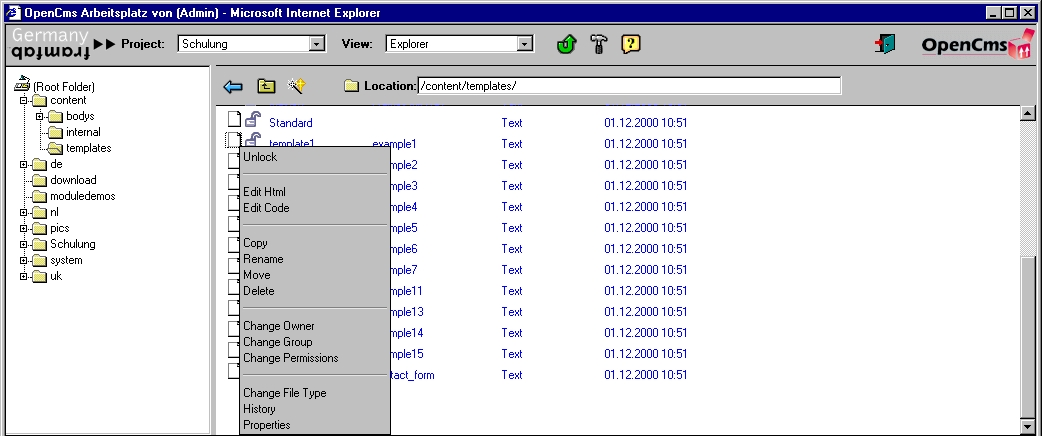
\includegraphics[width=\sgw]
                   {pics/templateMech/editcode}
\caption[select \textit{edit code}]
           {select \textit{edit code} from the context menu}
\label{editcode}
\end{center}
\end{figure}

Select {\name Edit Code} from the file's context menu to edit the
new file. The context menu is accessed by clicking on the new
file's icon (Figure~\ref{editcode}). This will start the Editor. A
template file is simply an XML file that contains XML and HTML
tags. The master template contains the definition of the frame-
and the contenttemplate. To accomplish this the template must
contain the following text :

% this should be used to include the examples but it didn't work :-(
%\begin{alltt}
%<?xml version="1.0" encoding="ISO-8859-1"?> 
<XMLTEMPLATE>
    <ELEMENTDEF name="contenttemplate">
        <CLASS>com.opencms.template.CmsXmlTemplate</CLASS>
        <TEMPLATE>/content/contenttemplates/contenttemplate1</TEMPLATE>
    </ELEMENTDEF>
    <ELEMENTDEF name="frametemplate">
        <CLASS>com.opencms.template.CmsXmlTemplate</CLASS>
        <TEMPLATE>/content/frametemplates/frametemplate1</TEMPLATE>
    </ELEMENTDEF>
<TEMPLATE> <ELEMENT name="frametemplate"/> </TEMPLATE>
</XMLTEMPLATE>

%\end{alltt}
\begin{verbatim}
<?xml version="1.0"?> <XMLTEMPLATE>
    <ELEMENTDEF name="contenttemplate">
        <CLASS>com.opencms.template.CmsXmlTemplate</CLASS>
        <TEMPLATE>/content/contenttemplates/contenttemplate1</TEMPLATE>
    </ELEMENTDEF>
    <ELEMENTDEF name="frametemplate">
        <CLASS>com.opencms.template.CmsXmlTemplate</CLASS>
        <TEMPLATE>/content/frametemplates/frametemplate1</TEMPLATE>
    </ELEMENTDEF>
<TEMPLATE> <ELEMENT name="frametemplate"/> </TEMPLATE>
</XMLTEMPLATE>
\end{verbatim}

You can either type in this text or copy and paste it into the
Editor. Exit the Editor and save the file by clicking on the icon
to the left that shows a floppy disk and a cross. Now create the
frametemplate1 in the directory {\dir /content/frametemplates}
with the text:
%<?xml version="1.0"?> <XMLTEMPLATE>
    <TEMPLATE><![CDATA[
        <html>
            <head>
                <title>The first templates</title>
            </head>
            <BODY >
                ]]><ELEMENT name="contenttemplate"/><![CDATA[
            </BODY>
        </html>]]>
    </TEMPLATE>
</XMLTEMPLATE>

\begin{verbatim}
<?xml version="1.0"?> <XMLTEMPLATE>
    <TEMPLATE><![CDATA[
        <html>
            <head>
                <title>The first templates</title>
            </head>
            <BODY >
                ]]><ELEMENT name="contenttemplate"/><![CDATA[
            </BODY>
        </html>]]>
    </TEMPLATE>
</XMLTEMPLATE>
\end{verbatim}

At last create the contenttemplate1 in {\dir
/content/contenttemplates} with this text:
%<?xml version="1.0" encoding="ISO-8859-1"?> <XMLTEMPLATE>
    <TEMPLATE><![CDATA[
            Hello World! <br>
        ]]><ELEMENT name="body"/>
    </TEMPLATE>
</XMLTEMPLATE>

\begin{verbatim}
<?xml version="1.0"?> <XMLTEMPLATE>
    <TEMPLATE><![CDATA[
            Hello World! <br>
        ]]><ELEMENT name="body"/>
    </TEMPLATE>
</XMLTEMPLATE>
\end{verbatim}

 The next step is to create a web page that uses the template set you just created. As mentioned before,
the page control file is the one that has to be clicked on to view a page in the Browser.
This file has to be created now. To do so, change to the Explorer view, go to the root folder
and use the wizard to create a new file. Select {\name Page} as the new file type. Enter the web
pages's name and title. The name is the name of the file and the title is the title that should
be shown when the page is requested. Select the master template for the new page from the
Template drop-down list, which displays the titles of the templates that can be found in the
{\dir /content/templates} directory (Figure~\ref{chooseMaster}).
The other fields in this dialog will be
discussed later. For the time being, they can retain their default values. Click
on the {\name Finish} button to create the new page.

\begin{figure}[hbt]
\begin{center}
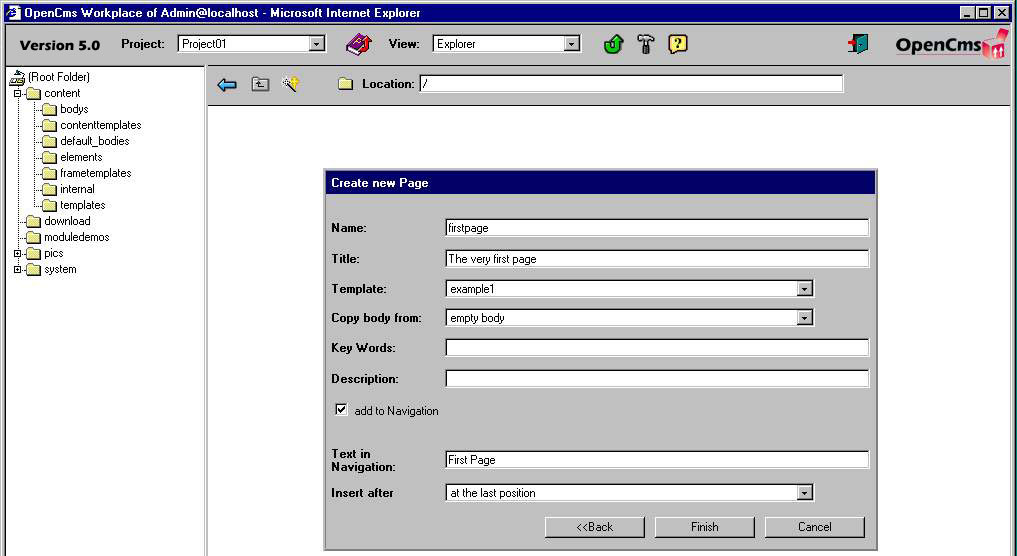
\includegraphics[width=\sgw]
                   {pics/templateMech/chooseMaster}
\caption[choose the master template]
           {The Template drop-down list displays the templates that are stored in the
            {\dir /content/templates} directory}
\label{chooseMaster}
\end{center}
\end{figure}

You can now view the page by clicking on it. A new browser window
will be opened in which the new page is displayed. The page shows
the {\name Hello, world!} text from the contenttemplate. The title
of the page is the title that was defined in the frametemplate.

\section{The body element}
%============================================================================
\subsection{A new frametemplate}

To achieve a separation of content and layout of a web site, the
content is normally inserted in a body element. So in this
example, we will modify the first frametemplate and use the body
element in the contenttemplate. A body element is a subtemplate,
the output of which is inserted in the contenttemplate in the
space where  the body element is placed. The frametemplate now
uses a method of the OpenCms system to set the title in the
template. To create the frametemplate you have to create a new
text file (frametemplate2) in the {\dir /content/frametemplates}
directory. Follow the steps to create a new template that are
described in the first example, and insert the following text in
your frametemplate:

%<?xml version="1.0" encoding="ISO-8859-1"?> <XMLTEMPLATE>
    <TEMPLATE><![CDATA[
        <html>
            <head>
                <title>]]><method name="getTitle"/><![CDATA[</title>
            </head>
                <BODY >
                    ]]><ELEMENT name="contenttemplate"/><![CDATA[
                </BODY>
        </html>]]>
    </TEMPLATE>
</XMLTEMPLATE>

\begin{verbatim}
<?xml version="1.0"?> <XMLTEMPLATE>
    <TEMPLATE><![CDATA[
        <html>
            <head>
                <title>]]><method name="getTitle"/><![CDATA[</title>
            </head>
                <BODY >
                    ]]><ELEMENT name="contenttemplate"/><![CDATA[
                </BODY>
        </html>]]>
    </TEMPLATE>
</XMLTEMPLATE>
\end{verbatim}
\index{getTitle}

Now you also need a new master template which uses the new
frametemplate2 and the old contenttemplate. Create it in {\dir
/content/templates} as described in the first example:

%<?xml version="1.0"?> <XMLTEMPLATE>
    <ELEMENTDEF name="contenttemplate">
        <CLASS>com.opencms.template.CmsXmlTemplate</CLASS>
        <TEMPLATE>/content/contenttemplates/contenttemplate1</TEMPLATE>
    </ELEMENTDEF>
    <ELEMENTDEF name="frametemplate">
        <CLASS>com.opencms.template.CmsXmlTemplate</CLASS>
        <TEMPLATE>/content/frametemplates/frametemplate2</TEMPLATE>
    </ELEMENTDEF>
<TEMPLATE> <ELEMENT name="frametemplate"/> </TEMPLATE>
</XMLTEMPLATE>

\begin{verbatim}
<?xml version="1.0"?> <XMLTEMPLATE>
    <ELEMENTDEF name="contenttemplate">
        <CLASS>com.opencms.template.CmsXmlTemplate</CLASS>
        <TEMPLATE>/content/contenttemplates/contenttemplate1</TEMPLATE>
    </ELEMENTDEF>
    <ELEMENTDEF name="frametemplate">
        <CLASS>com.opencms.template.CmsXmlTemplate</CLASS>
        <TEMPLATE>/content/frametemplates/frametemplate2</TEMPLATE>
    </ELEMENTDEF>
<TEMPLATE> <ELEMENT name="frametemplate"/> </TEMPLATE>
</XMLTEMPLATE>
\end{verbatim}

\subsection{The body template}
Create a new page in the root folder and select the title of the
new template from the drop-down list. For example, if you have
defined the title of the template as template2, this text should
appear in the drop-down list. Enter a title and name for your new
page, and select {\name Finish} to create the page
(Figure~\ref{selectTitle}).

\begin{figure}[hbt]
\begin{center}
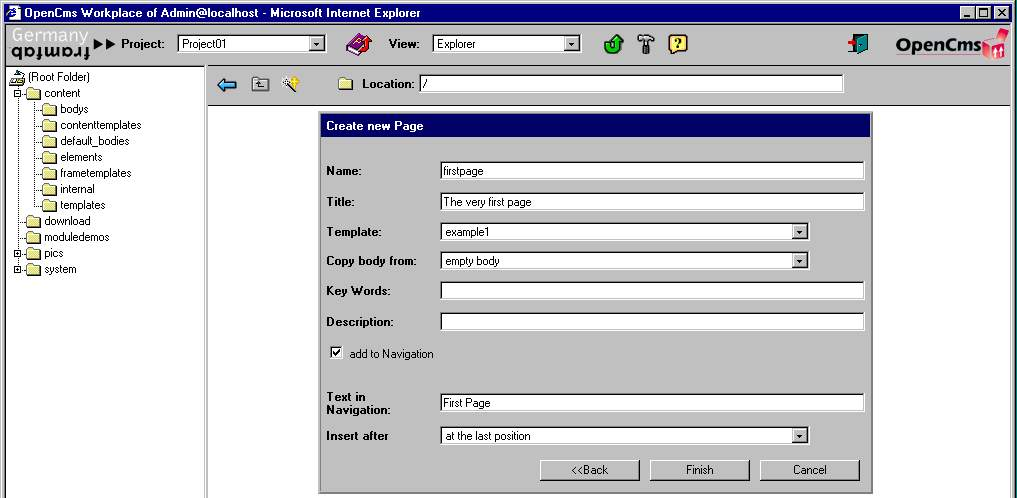
\includegraphics[width=\sgw]
                   {pics/templateMech/setTitle}
\caption[select the title of the template]
           {Select the title of the new template when creating the page}
\label{selectTitle}
\end{center}
\end{figure}

Before we take a look at the new page, we will use the HTML Editor
to add text to the body element. To edit the page with the HTML
Editor select {\name Edit Page} from the new page's context
menu.(Figure~\ref{EditPage})

\begin{figure}[hbt]
\begin{center}
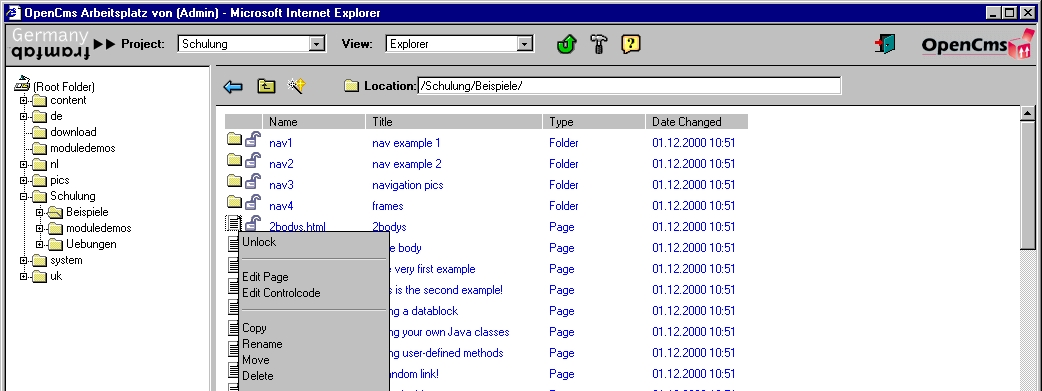
\includegraphics[width=\sgw]
                   {pics/templateMech/editPage}
\caption[{\name Edit Page}]
           {Select {\name Edit Page} from the context menu to edit the page in the HTML Editor}
\label{EditPage}
\end{center}
\end{figure}

The Editor is a WYSIWYG editor that provides standard HTML file
editing functionality. You can select the font style and size,
insert pictures, and so on. Entering text in the editor inserts it
in the new page's body element.(Figure~\ref{EditBody})

\begin{figure}[hbt]
\begin{center}
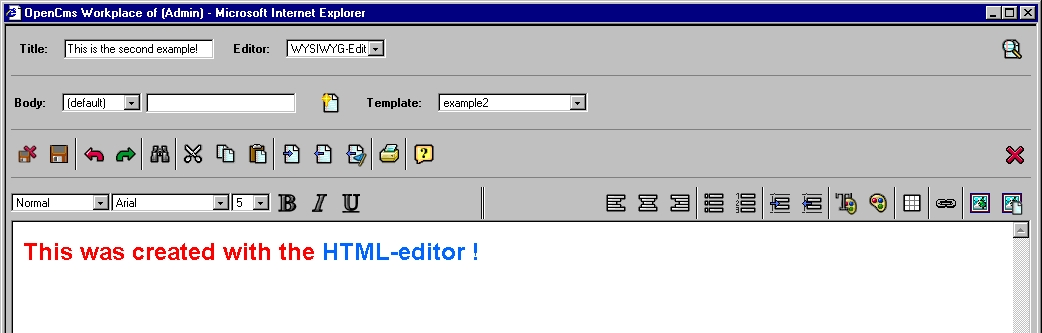
\includegraphics[width=\sgw]
                   {pics/templateMech/HTMLEdit}
\caption[Edit the body]
           {Edit the body with the HTML Editor}
\label{EditBody}
\end{center}
\end{figure}

After you have entered your text, close the Editor by clicking on the  {\name Save and Exit} icon
to the left. Have a look at the new page by clicking on its name. If you entered the text in
the above example, the page will look like Figure~\ref{ThisOutp}

\begin{figure}[hbt]
\begin{center}
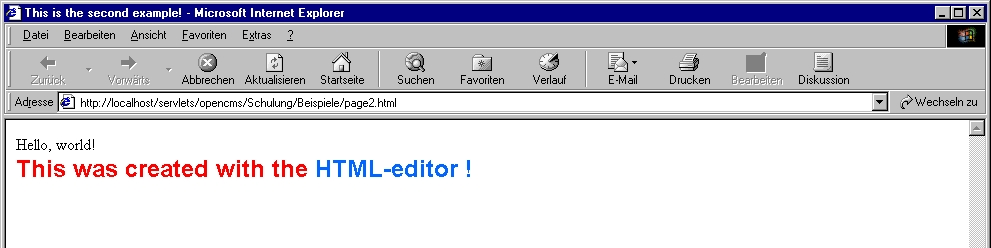
\includegraphics[width=\sgw]
                   {pics/templateMech/ThisOutput}
\caption[The output of the second page]
           {The output of the second page}
\label{ThisOutp}
\end{center}
\end{figure}

\subsection{The element-tag}
As you can see, the first part of the text ({\name Hello, world!})
still comes from the contenttemplate, but the second part, witch
was created with the help of the WYSIWYG-editor, comes from the
body element. You can see in the contenttemplate, that the body
template is inserted via the ELEMENT-tag:

\begin{xml}
...\\
\xtaba Hello, world!<br>\\
\xtaba ]]><ELEMENT name="body"/>\\
...\\
\end{xml}

Here, the element with the name {\name body} is inserted after the
{\name Hello, world!} text. The assignment of the element  {\name
body} to the body template in the {\dir /content/bodys} directory
is made in the page control file.

Another difference to the earlier example is the fact, that the
title which was typed in when creating the page, is now correct
shown in the Browser. This is because of the usage of the {\it
getTitle()}-method in the frametemplate. OpenCms provides a number
of standard methods that can be used when creating
a template. The methods are defined in the\\
\textit{com.opencms.template.CmsXmlTmplate} class which is
assigned to the master template per default in the page control file.
As you can see, the usage of standard methods is quite simple.

\begin{xml}
  <TITLE>]]><method name="getTitle"/><![CDATA[</TITLE>
\end{xml}

The method-tag is a special tag which allows to call functions from a template. The return
value of the method (in this case the correct title of the page) is inserted into the page when
the template is processed. Other standard methods will be discussed later in this document.

\section{Further Elementes}
%============================================================================
\subsection{A master template with a table}

We will now go a little step further and come closer to the recommended layout of an OpenCms
web site. Normally, an OpenCms web site is more or less designed like
Figure~\ref{MasterAndElems}.

\begin{figure}[hbt]
\begin{center}
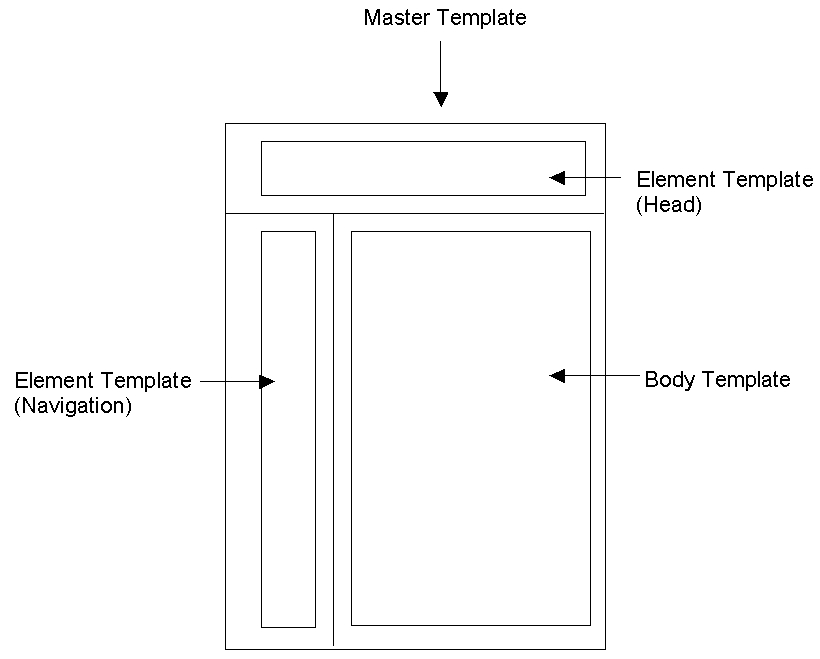
\includegraphics[width=\sgw]
                   {pics/templateMech/MasterAndElementes}
\caption[Master and Elementes]
           {Master and Elementes}
\label{MasterAndElems}
\end{center}
\end{figure}

A head-section for logos and things like that, an element for the
navigation and a content area for the content. This layout can for
example be realized with a table defined in the frametemplate and
three elements which are inserted. To  create a page with this
layout, you should first create the frametemplate3 with the table
in the {\dir /content/frametemplate} directory.  The creation can
be done similar to the way we did it before. You can then add the
following code to the frametemplate3:
%<XMLTEMPLATE>
<TEMPLATE><![CDATA[
    <HTML>
        <HEAD>
            <TITLE>]]><method name="getTitle"/><![CDATA[</TITLE>
        </HEAD>
        <BODY>
            <TABLE border width="100%" height="100%">
                <TR height="30%">
                    <TH colspan=2 width="100%" align="center">
                        The Head section
                    </TH>
                </TR>
                <TR height="70%">
                    <TD width="20%" align="center" valign="top">
                        Navigation
                    </TD>
                    <TD width="80%" align="center">
                        ]]><ELEMENT name="contenttemplate"/><![CDATA[
                    </TD>
                </TR>
            </TABLE>
        </BODY>
    </HTML>]]>
</TEMPLATE>
</XMLTEMPLATE>

\begin{verbatim}
<XMLTEMPLATE>
<TEMPLATE><![CDATA[
    <HTML>
        <HEAD>
            <TITLE>]]><method name="getTitle"/><![CDATA[</TITLE>
        </HEAD>
        <BODY>
            <TABLE border width="100%" height="100%">
                <TR height="30%">
                    <TH colspan=2 width="100%" align="center">
                        The Head section
                    </TH>
                </TR>
                <TR height="70%">
                    <TD width="20%" align="center" valign="top">
                        Navigation
                    </TD>
                    <TD width="80%" align="center">
                        ]]><ELEMENT name="contenttemplate"/><![CDATA[
                    </TD>
                </TR>
            </TABLE>
        </BODY>
    </HTML>]]>
</TEMPLATE>
</XMLTEMPLATE>
\end{verbatim}

You also need a new mastertemplate in {\dir /content/templates}
where you use the new frametemplate and an empty contenttemplate:
%<?xml version="1.0" encoding="ISO-8859-1"?> 
<XMLTEMPLATE>
    <ELEMENTDEF name="contenttemplate">
        <CLASS>com.opencms.template.CmsXmlTemplate</CLASS>
        <TEMPLATE>/content/contenttemplates/empty</TEMPLATE>
    </ELEMENTDEF>
    <ELEMENTDEF name="frametemplate">
        <CLASS>com.opencms.template.CmsXmlTemplate</CLASS>
        <TEMPLATE>/content/frametemplates/frametemplate3</TEMPLATE>
    </ELEMENTDEF>
<TEMPLATE> <ELEMENT name="frametemplate"/> </TEMPLATE>
</XMLTEMPLATE>

\begin{verbatim}
<?xml version="1.0"?> <XMLTEMPLATE>
    <ELEMENTDEF name="contenttemplate">
        <CLASS>com.opencms.template.CmsXmlTemplate</CLASS>
        <TEMPLATE>/content/contenttemplates/empty</TEMPLATE>
    </ELEMENTDEF>
    <ELEMENTDEF name="frametemplate">
        <CLASS>com.opencms.template.CmsXmlTemplate</CLASS>
        <TEMPLATE>/content/frametemplates/frametemplate3</TEMPLATE>
    </ELEMENTDEF>
<TEMPLATE> <ELEMENT name="frametemplate"/> </TEMPLATE>
</XMLTEMPLATE>
\end{verbatim}


As you can see, the text for the head-section and the
navigation-section is just inserted dircetly in the frametemplate,
but the content is inserted as an element. The empty
contenttemplate just inserts the body element. Please create a new
page witch uses the new master template with the wizard and edit
the body with the WYSIWYG-editor so that you can see some output.
Afterwards the output could look like Figure~\ref{MasterEl}.

\begin{figure}[hbt]
\begin{center}
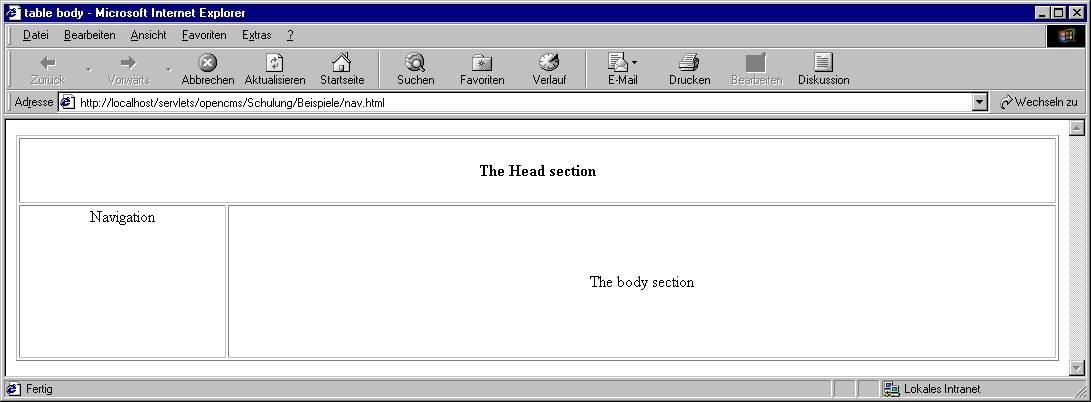
\includegraphics[width=\sgw]
                   {pics/templateMech/simpleTable}
\caption[Master and subelementes]
           {Master and subelementes}
\label{MasterEl}
\end{center}
\end{figure}

This example should also give a little insight in how to handle
standard HTML features as e.g. tables and the XML tags together.
You can now try to change the layout of the page and edit the
frametemplate and the contenttemplate. Another thing that you
should try is to "insert" a second body in you web site. This is
very easy to do. You simply have to create a second page with the
wizard and choose the same master template. You might have noticed
that you can specify wether or not your page should included in
the navigation, and at what position this should be.

\subsection{The default navigation class in opencms}

The navigation concept is based on a representation of files and
folders of the VFS of OpenCms. To show a file or a folder in the
navigation two properties must be added to the resource, the
navigation position and the navigation text.

To build a dynamic navigation you need to define some files or
folders, by entering the position of Navigation and navigation
text in dialog box, while creating a file or folder. If there is a
group of Navigation entries belonging together then a folder must
be defined in which the Navigation entries are represented by HTML
files.

Per default a link of a folder of navigation is consisting of the
folder path with index.html file, e.g if there is a folder as
navigation entry {\dir /news/sport/} then the link of this entry
in navigation is {\dir /news/sport/index.html}. It means that the
required index.html file must not be included in the navigation,
because it is automatically added via the folder itself. If
index.html file is not existing in this folder then the link of
naviagtion would be the current url. If the default name schould
be changed index.html to another name (e.g. news.html) then a
property {\name NavIndex} must be add to the folder that is used
as navigation entry.

There are some methods in the CmsXmlNav class that are used to
build a simple navigation. If there is another design of
navigation that cannot be build with this navigation class then a
new class must be written and CmsXmlNav must be extended.

To display the navigation, an element {\name nav} must be defined
in the frametemplate of the files. In the element definition of
this element, the class CmsXmlNav and a template file {\name
navigation} must be defined. The template of this element is used
to define the required HTML-code to build the Navigation. Example:
First the frametemplate:

%<?xml version="1.0"?>
<XMLTEMPLATE>
<TEMPLATE><![CDATA[
    <HTML>
    <HEAD>
        <TITLE>]]><method name="getTitle"/><![CDATA[</TITLE>
    </HEAD>
    <BODY>
    <TABLE border width="100\%" height="100\%">
        <TR height="30\%">
        <TH colspan=2 width="100\%" align="center">
            The Head section
        </TH>
        </TR>
        <TR height="70\%">
        <TD width="20\%" align="center" valign="top">
            ]]><element name="nav"/><![CDATA[
        </TD>
        <TD width="80\%" align="center">
            ]]><element name="contenttemplate"/><![CDATA[
        </TD>
    </TR>
    </TABLE>
    </BODY>
    </HTML>]]>
</TEMPLATE>

<ELEMENTDEF name="nav">
    <CLASS>com.opencms.defaults.CmsXmlNav</CLASS>
    <TEMPLATE>/content/elements/navigation</TEMPLATE>
</ELEMENTDEF>

</XMLTEMPLATE>

\begin{verbatim}
<?xml version="1.0"?> <XMLTEMPLATE> <TEMPLATE><![CDATA[
    <HTML>
    <HEAD>
        <TITLE>]]><method name="getTitle"/><![CDATA[</TITLE>
    </HEAD>
    <BODY>
    <TABLE border width="100\%" height="100\%">
        <TR height="30\%">
        <TH colspan=2 width="100\%" align="center">
            The Head section
        </TH>
        </TR>
        <TR height="70\%">
        <TD width="20\%" align="center" valign="top">
            ]]><element name="nav"/><![CDATA[
        </TD>
        <TD width="80\%" align="center">
            ]]><element name="contenttemplate"/><![CDATA[
        </TD>
    </TR>
    </TABLE>
    </BODY>
    </HTML>]]>
</TEMPLATE>

<ELEMENTDEF name="nav">
    <CLASS>com.opencms.defaults.CmsXmlNav</CLASS>
    <TEMPLATE>/content/elements/navigation</TEMPLATE>
</ELEMENTDEF>

</XMLTEMPLATE>
\end{verbatim}
\index{ELEMENTDEF}
\index{element}
\index{getTitle}

Now the definition of the navigation element in {\dir
/content/elements/}

%<?xml version="1.0" encoding="ISO-8859-1"?> <XMLTEMPLATE>

<naventry>
    <![CDATA[
    <tr>
     <td>
      <a href="]]><process>navlink</process><![CDATA[">
             ]]><process>navtext</process><![CDATA[
      </a>
     </td>
    </tr>
    ]]>
</naventry>

<navcurrent>
    <![CDATA[
    <tr>
     <td>
       ]]><process>navtext</process><![CDATA[
     </td>
    </tr>
    ]]>
</navcurrent>

<TEMPLATE>
    <![CDATA[
    <TABLE border width="100\%" height="100\%">
      ]]><method name="getNavCurrent"/><![CDATA[
    </TABLE>
    ]]>
</TEMPLATE>

</XMLTEMPLATE>

\begin{verbatim}
<?xml version="1.0"?> <XMLTEMPLATE>

<naventry>
    <![CDATA[
    <tr>
     <td>
      <a href="]]><process>navlink</process><![CDATA[">
             ]]><process>navtext</process><![CDATA[
      </a>
     </td>
    </tr>
    ]]>
</naventry>

<navcurrent>
    <![CDATA[
    <tr>
     <td>
       ]]><process>navtext</process><![CDATA[
     </td>
    </tr>
    ]]>
</navcurrent>
<TEMPLATE>
    <![CDATA[
    <TABLE border width="100\%" height="100\%">
      ]]><method name="getNavCurrent"/><![CDATA[
    </TABLE>
    ]]>
</TEMPLATE>
</XMLTEMPLATE>
\end{verbatim}
\index{ELEMENTDEF}
\index{element}
\index{getNavCurrent}

There are several definitions of data blocks and one method used in this example. The definition of {\name naventry} datablock is compulsory, otherwise no element of navigation would be shown. It is used to generate navigation entry.The {\name navcurrent} data block is to show the element of current navigation position in a different way than the other navigation elements. \\
The method {\name getNavCurrent} is a method defined in CmsXmlNav class and gets the navigation from current folder. \\

The following methods defined in CmsXmlNav class could be used to build different types of Navigation. Here is the definition of the methods, tools and datablocks defined in CmsXmlNav class: \\

Data blocks that must be defined in the tamplates that is managed by CmsXmlNav: \\

- navtext \index{navtext} \\
- navlink \index{navlink} \\
- naventry \index{naventry} \\
- navcurrent \index{navcurrent} \\
- navstart \index{navstart} \\
- navend \index{navend} \\

Additional data blocks that could be used as useful data blocks in a navigation structure: \\

- navlevel \index{navlevel} \\
- navcount \index{navcount} \\

Methods that are defined in CmsXmlNav: \\

- getNavCurrent \index{getNavCurrent} \\
- getNavFold \index{getNavFold} \\
- getNavTree \index{getNavTree} \\
- getNavParent \index{getNavParent} \\
- getNavRoot \index{getNavRoot} \\


Additional methods that can be used as helpful tools in template: \\

- getFolderCurrent \index{getFolderCurrent} \\
- getFolderParent \index{getFolderParent} \\
- getFolderRoot \index{getFolderRoot} \\
- getPropertyCurrent \index{getPropertyCurrent} \\
- getPropertyParent \index{getPropertyParent} \\
- getPropertyRoot \index{getPropertyRoot} \\
- getPropertyUri \index{getPropertyUri} \\
\subsubsection{Definition of data blocks:}
\subsubsection{- navtext:} \index{navtext}
  This data block is used to display the navigation text. The navigation text is defined in {\name NavText} property of corresponding file or folder. \\

\subsubsection{- navlink:} \index{navlink}
  This data block defines the path of the corresponding navigation entry, This is the path of the file or folder.\\

\subsubsection{- naventry:} \index{}
  The definition of this data block is compulsory because this data block defines the layout of a navigation entry. For each navigation entry this data block is used. Example: \\

  \begin{xml}
  <naventry> \\
  <![CDATA[ \\
  <tr> \\
  \xtaba <td> \\
  \xtabb   <a href="]]><process>navlink</process><![CDATA[ class="nav" target="\_blank"> \\
  \xtabc      ]]><process>navtext</process><![CDATA[ \\
  \xtabb   </a> \\
  \xtaba </td> \\
  </tr> \\
  ]]> \\
  </naventry> \\
  \end{xml}

\subsubsection{- navcurrent:} \index{navcurrent}
  With the definition of this data block, the layout of the current navigation position is set.If this data block is not defined, the {\tag <naventry>} datablock is used. Example: \\

  \begin{xml}
  <navcurrent> \\
  <![CDATA[ \\
  <tr> \\
  \xtaba <td> \\
  \xtabb   <font color="red">]]><process>navtext</process><![CDATA[</font> \\
  \xtaba </td> \\
  </tr> \\
  ]]> \\
  </navcurrent> \\
  \end{xml}

\subsubsection{- navstart and navend:} \index{navstart} \index{navend}
  These data blocks are used in nested navigation system, so if the method {\name getNavFold} or {\name getNavTree} is used then these data blocks could be used to format the navigation. The methods mentioned above are working recursive and after each call these datablocks are used to format the navigation entries, e.g. a definition of the data block {\tag <navstart>} as a {\tag <ul>} tag and the {\tag <navend>} data block as a {\tag </ul>} tag, so by recursive call of the method then a nested {\tag <ul>} ... {\tag </ul>} list is created. Example: \\

  \begin{xml}
  <navstart><![CDATA[<ul>]]></navstart> \\
  <naventry><![CDATA[ \\
    \xtaba <li> \\
    \xtaba <a href="]]><process>navlink</process><![CDATA["> \\
    \xtabb ]]><process>navtext</process><![CDATA[ \\
    \xtaba </a>]]> \\
  </naventry> \\
  <navcurrent><![CDATA[<li>]]><process>navtext</process></navcurrent> \\
  <navend><![CDATA[</ul>]]></navend> \\
  \end{xml}

  If the {\tag <navstart>} and {\tag <navend>} are not defined then they are ignored. \\

\subsubsection{- navlevel:} \index{navlevel}
  This data block contains the depth of the navigation entry. This data block could be used in nested navigation system. e.g. the definition a group of style sheets depending on the depth of navigation. Example: \\

  \begin{xml}
  <navstart><![CDATA[<ul>]]></navstart> \\
  <naventry><![CDATA[ \\
  \xtaba <li class="nav\_]]><process>navlevel</process><![CDATA["> \\
  \xtaba <a class="nav\_]]><process>navlevel</process><![CDATA[" \\
  \xtaba href="]]><process>navlink</process><![CDATA["> \\
  \xtabb ]]><process>navtext</process><![CDATA[ \\
  \xtaba </a>]]> \\
  </naventry> \\
  <navcurrent><![CDATA[ \\
      <li class="nav\_]]><process>navlevel</process><![CDATA["> \\
      ]]><process>navtext</process> \\
  </navcurrent>\\
  <navend><![CDATA[</ul>]]></navend>\\
  \end{xml}

  With the <navlevel> the depth of navigation entry is determined and with a corresponding definition of the style sheet in a .css file (e.g. nav\_1{....},nav\_2{....},nav\_3{....}, ....) each level of the navigation can be formatted in different way. \\

  It is very important to know that if the level number in a method is given as parameter then the real depth would be calculated from the difference number of the depth of currentfolder and the given depth as parameter in the method. \\

\subsubsection{- navcount:} \index{navcount}
  An additional data block that returns the number of navigation entries in the navigation. \\
\subsubsection{Definition of Methods:}
\subsubsection{- getNavCurrent:} \index{getNavCurrent}
  This method gets the Navigation of current folder, This method uses {\name naventry} and {\name navcurrent} data blocks.\\

\subsubsection{- getNavFold:} \index{getNavFold}
  This method gets the navigation of specified folder. If an entry is clicked then the navigation of that entry will be added to current navigation. Because of folding functionality this method is called getNavFold. \\
  This method uses {\tag <naventry>}, {\tag <navcurrent>}, {\tag <navstart>} and {\tag <navend>} data blocks. \\

  This method could get a level and depth as parameter in the following form: \\
  {\tag <method name="getNavFold/>} \\
  {\tag <method name="getNavFold>level</method>} \\

  The level parameter defines the starting point of Navigation from which the navigation must be constructed. For example if the current folder is {\dir /news/sport/football/liga/first/} and the method definition is {\tag <method name="getNavFold>2</method>} then the starting point of navigation would be {\dir /sport/} folder and all elements starting from {\tag /sport/} folder would be displayed.\\

  If there is no level as parameter defined then the starting point is set to the root folder. \\

\subsubsection{- getNavtree:} \index{getNavtree}
  This method gets the navigation starting from a folder and shows all navigation recursive as a tree. Therefore this method is called {\name getNavTree}. \\

  This method can get a level and depth as parameter in the following form: \\
  {\tag <method name="getNavTree/>} \\
  {\tag <method name="getNavTree>level</method>} \\
  {\tag <method name="getNavTree>level,depth</method>} \\

  The level parameter defines the starting point of Navigation from which the navigation must be constructed. For example if the current folder is {\dir /news/sport/football/liga/first/} and the method definition is {\tag <method name="getNavTree>2</method>} then the starting point of navigation would be {\dir /sport/} folder and all elements starting from {\dir /sport/} folder would be displayed. \\

  If there is no level as parameter defined then the starting point is set to the root folder. \\

  The depth parameter defines how many levels of folders must be displayed in the navigation tree. For example if the current Folder is {\dir /news/sport/football/liga/first/} and the method definition is {\tag <method name="getNavTree>1,3</method>} then the starting point of navigation would be {\dir /news/} and it ends in folder {\dir /news/sport/football/}. \\

\subsubsection{- getNavParent:} \index{getNavParent}
  This method gets the navigation from parent folder depending on the given parameter. For example if the current Folder is {\dir /news/sport/football/liga/first/} and the method definition is {\tag <method name="getNavParent>2</method>} then the navigation in folder {\dir /news/sport/football/} would be displayed (two level back). This method gets only one parameter, if there is no given parameter then the navigation in current folder is displayed. If the number given as parameter exceeded from the sum of the folders then the root folder is chosen. \\

\subsubsection{- getNavRoot:} \index{getNavRoot}
  This method gets the navigation starting from root folder depending on the given parameter. For example if the current folder is {\dir /news/sport/football/liga/first/} and the method definition is {\tag <method name="getNavRoot>2</method>} then the navigation in folder {\dir /news/sport/} would be displayed (second level starting from root). This method gets only one parameter, if there is no given parameter then the navigation in current folder is choosen. If the number given as parameter exceeded from sum of the folders then the current folder is chosen. \\

\subsubsection{- getFolderCurrent:} \index{getFolderCurrent}
  This method gets the current folder, this method has the same functionality of method {\name getPathUri} in CmsXmlTemplate class. \\

\subsubsection{- getFolderParent:} \index{getFolderParent}
  This method gets the parent folder depending on the given parameter. For example if the current folder is {\dir /news/sport/football/liga/first/} and the method definition is {\tag <method name="getFolderParent>2</method>} then the folder returned by this method would be {\dir /news/sport/football/}. This method gets only one parameter, if there is no given parameter then the current folder is returned. If the number given as parameter exceeded from the sum of the folders then the root folder is returned. \\

\subsubsection{- getFolderRoot:} \index{getFolderRoot}
  This method gets the folder starting from root folder depending on the given parameter. For example if the current folder is {\dir /news/sport/football/liga/first/} and the method definition is {\tag <method name="getFolderRoot>2</method>} then the folder {\dir /news/sport/} would be displayed (second level starting from root). This method gets only one parameter, if there is no given parameter then the root folder is returned. If the number given as parameter exceeded from sum of the folders then the current folder is returned. \\

\subsubsection{- getPropertyCurrent:} \index{getPropertyCurrent}
  This method gets the property of current folder. This method is used in the following format:\\
  {\tag <method name="getProperyCurrent">property</method>} \\
  property is the name of property that must be read. If there is no such property name then nothing is returned. \\

\subsubsection{- getPropertyParent:} \index{getPropertyParent}
  This method gets the property of parent folder, depending on the given number. This method is used in the following format:\\
  {\tag <method name="getPropertyParent">level,property</method>} \\
  property is the name of property that must be read. If there is no such property name then nothing would be returned. \\
  level is the number of parent folder, e.g. if the current folder is {\dir /news/sport/football/liga/first/} and the method definition is {\tag <method name="getPropertyParent">2,NavPic</method>} then the value of {\name NavPic} property of {\dir /news/sport/football/} folder would be returned by this method.If the number given as parameter exceeded from the sum of the folders then the specified property of root folder is read. \\

\subsubsection{- getPropertyRoot:} \index{getPropertyRoot}
  This method gets the property of the folder starting from root and depending on the given number. This method is used in the following format:\\
  {\tag <method name="getPropertyRoot">level,property</method>} \\
  property is the name of property that must be read. If there is no such property name then nothing is returned.\\
  level is the number of parent folder, e.g. if the current folder is {\dir /news/sport/football/liga/first/} and the definition of method is {\tag <method name="getPropertyRoot">2,NavPic</method>} then the value of {\name NavPic} property of {\dir /news/sport/} folder would be returned by this method. If the number given as parameter exceeded from sum of the folders then the property of current folder is returned. \\

\subsubsection{- getPropertyUri:} \index{getPropertyUri}
  This method returns the specified property of current uri. This method is used in the following format:\\
  {\tag <method name="getProperyUri">property</method>} \\
  property is the name of property that must be read. If there is no such property name then nothing is returned. \\


It is very usual to use an image instead of Text in navigation, therefore here is an example that uses image instead of using a navigation text: \\

\begin{xml}
<?xml version="1.0"?> \\
<XMLTEMPLATE> \\

<naventry> \\
<![CDATA[ \\
<tr> \\
\xtaba <td> \\
\xtabb   <a href="]]><process>navlink</process><![CDATA[" \\
\xtabc   onmouseover="JavaScript:document.image\_ \\
\xtabc   ]]><process>count</process><![CDATA[.value= \\
\xtabc   '/pics/templates/]]><process>navtext</process> \\
\xtabc   <![CDATA[\_light.gif'" \\
\xtabc   onmouseout="JavaScript:document.image\_]]> \\
\xtabc   <process>count</process><![CDATA[.value= \\
\xtabc   '/pics/templates/]]><process>navtext</process><![CDATA[.gif'"> \\
\xtabc   <img name="image\_]]><process>count</process><![CDATA[" \\
\xtabc   src="/pics/templates/ \\
\xtabc   ]]><process>navtext</process><![CDATA[.gif"> \\
\xtabb   </a> \\
\xtaba </td> \\
</tr> \\
]]> \\
</naventry> \\

<navcurrent> \\
<![CDATA[ \\
<tr> \\
\xtaba  <td> \\
\xtabb    <img src="/pics/templates/]]><process>navtext</process><![CDATA[.gif"> \\
\xtaba  </td> \\
</tr> \\
]]> \\
</navcurrent> \\

<TEMPLATE> \\
<![CDATA[ \\
<TABLE border width="100\%" height="100\%"> \\
\xtaba  ]]><method name="getNavCurrent"/><![CDATA[ \\
</TABLE> \\
]]> \\
</TEMPLATE> \\

</XMLTEMPLATE> \\
\end{xml}


To build a navigation using images instead of text, an image name must be written in {\name NavText} property. To have the mouse over effect and mouse out effect, it is needed to have another pictures with the same name but with a suffix, so the picture would be found and replaced with javascript. In the above example first of all the image name would be constructed with the count data block (so image\_1, image\_2,.... would be generated) then by mouse over the corresponding image would be replaced with the image with the same name but with the suffix of {\name \_light}, so if the picture name is {\name nav.gif} then by mouse over picture would be replaced with nav\_light.gif and by mouse out nav.gif. \\


\section{Templates and directories}
%============================================================================
\subsection{The XML structure of a template}
\index{XML}
XML is a markup language, which is just like HTML defined by SGML and is used to store content
in a sturctured way.  The main difference, and this is the part which is important when using
XML in OpenCms, ist that one is able to define his own tags. By that, it is possible to achieve
a separation between content and layout.
While HTML allows to define how something should be displayed allows XML to define items that
belong ligically together.
For example, it is possible to define blocks of surnames, adresses etc..
XML is a powerfull markup language, but you don�t need to know much about it for understanding
the template mechanism, and there are only a few XML-tags which are used by OpenCms. OpenCms
uses XML to deposit HTML fragments single and sturctured. These fragments can then be fetched
specifically and used dynamically.
From the technical site of view, there is no difference between the master and the body (sub)
templates. Both are XML-files with the same syntax. The difference is more a logical one.The
following section explains the structure of a template file.
Below is the general framework of a template file:
\index{XML-tags}
\begin{xml}
<?xml version="1.0"?>\\
<XMLTEMPLATE>\\
<!-- user-defined datablocks or elementdefintions -->\\
<TEMPLATE>\\
\xtaba <![CDATA[\\
\xtaba   <!-- HTML-code -->\\
\xtaba   ]]> <XML-TAGS> [![CDATA[\\
\xtaba   <!-- the  HTML-code  continues here... -->\\
\xtaba
\xtaba      ]]>\\
</TEMPLATE>\\
<!-- user-defined datablocks or elementdefinitions -->\\
</XMLTEMPLATE>\\
\end{xml}
\index{XMLTEMPLATE}
\index{TEMPLATE}

The first line determines the type of the document and must be placed at the very beginning of
the document. Leading spaces are not allowed. The whole template is enclosed between
{\tag <XMLTEMPLATE>} tags. Inside this tag the template is defined between the start
{\tag <TEMPLATE>} tag and
the end {\tag </TEMPLATE>} tag. HTML code can be placed in the template between the CDATA tags,
which starts with
{\tag <![CDATA[ } and ends with {\tag ]]>}.
Everything between CDATA tags is ignored by the XML
parser and directly streamed to the output. XML tags that are used in the template must be
placed outside of the {\tag CDATA} tags.  Examples for XML tags that can be used have been shown
in the first examples. You will primarily place process, element, or method tags in your document.
Outside the template tags and inside the {\name xmltemplate} tags you can place data blocks
or element definitions.
\index{CDATA}

\subsection{Directory structure}

The OpenCms system creates a standard directory structure for
every new project in the virtual file system. The templates, body
templates, page control files etc. are stored in separate
directories. If you create a new file of the type {\name Page}
within a project, only the page control file is created in the
directory you are actually in. At the same time there is
automatically a body-template with the same name created in the
{\dir /content/bodys directory}. If you click on the page control
file and choose {\name Edit Page} from the context menue, you
actually edit the body in the {\dir /content/bodys directory} with
the WYSIWYG-editor. You can check this out by looking at both
files with the source-code-editor after you have changed
something, but you should never change the files in body directory
directly.

\subsection{The subdirectorys of the content folder}
\index{content}

\subsubsection{- templates:} \index{templates}

In the directory {\dir /content/templates} are the definitions for
the different combinations of frame- and contenttemplates. These
files have always the same structure as you have seen in the
examples so far. The only things that can be changed are the names
of the two templates (only names not the path!). Never add any
other html or xml stuff here.

\subsubsection{- frametemplates:} \index{frametemplates}

In the frametemplates the design of the frame is build. e.g. it
can contain the navigation and an head element. There is always
the area where the contenttemplate is included which was defined
in the master template.

\subsubsection{- contenttemplates:} \index{contenttemplates}

The contenttemplates are subframes which include the body element
and maybe other elements.

\subsubsection{- bodys:} \index{bodys}

This folder is for internal use only. It contains the above
mentioned body elements.

\subsubsection{- default\_bodies:} \index{defaultbodies}

In this folder you can store some bodies which you use often. When
you create a new page you can chose one of these bodies to be
copied in your new pagebody.

\subsubsection{- internal:} \index{internal}

This directory is not used any more. It is still there for
compatibility reasons and its job is now taken over by the
elements folder.

\subsubsection{- elements:} \index{elements}

Here you can store your dynamic elements. A element is dynamic if
it don't use the standard class CmsXmlTemplate. For Example the
navigation element.


\begin{figure}[hbt]
\begin{center}
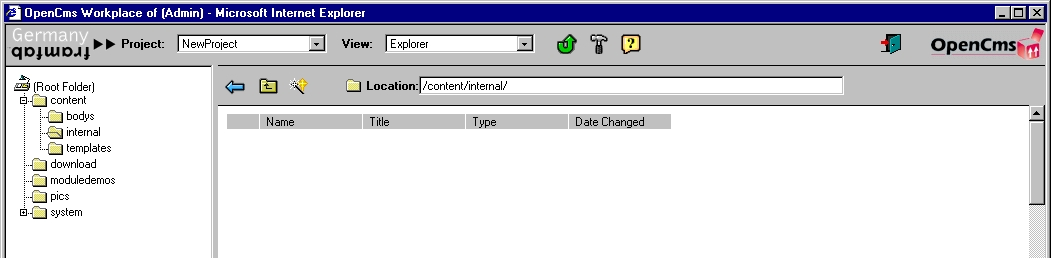
\includegraphics[width=\sgw]
                   {pics/templateMech/StandardDirectories}
\caption[Standard directories]
           {The Standard directories for a new project}
\label{StDir}
\end{center}
\end{figure}

Table~\ref{directTab1} shows which files are stored in the different directories.

\begin{table}
\begin{tabular}{|l|p{0.55\linewidth}|}
\hline
Directory &
Files stored in the Directory \\
/content &
Parent directory for the directories that take up the template files.\\
/download&
Files that can be downloaded.\\
/pics&
Picture files used in web sites\\
/system &
Parent directory for several directories that contain workplace templates and
configuration files for the system\\
/system/workplace/action&
Executable files like login, copy etc.\\
/system/workplace/administration&
Subdirectories for every Item in the Administration view.\\
/system/workplace/config&
The language files that are stored in subdirectories for every
language, and different configuration files.\\
/system/workplace/css&
The used style sheets.\\
/system/workplace/help&
The help system.\\
/system/workplace/pics&
The pictures that are used to create the workplace.\\
/system/workplace/templates&
The templates that are used to create the workplace.\\
\hline
\end{tabular}
\caption[Standard directories] {Standard directories}
\label{directTab1}
\end{table}

\subsection{Using Data Blocks}
Up to here, you got an overview over the templatemechanism, but many things which have already
been used have not been explained. We will now go one step back and take a look at some earlier
examples and the basic structures of the template mechanism.

In this example you will learn how to use data blocks in a
template. A data block is a named block of text that can contain
XML and HTML code. We will change the earlier example by putting
the {\name Hello, world!} text into a data block with the name
{\name message.} To create the new contenttemplate, create a new
text file named contenttemplate2 in the {\dir
/content/contenttemplates} directory with the following text:
\index{data blocks}

%<?xml version="1.0"?>
<XMLTEMPLATE>
    <MESSAGE><![CDATA[Hello world!]]></MESSAGE>
    <TEMPLATE><![CDATA[
            ]]><PROCESS>message</PROCESS><![CDATA[ <br>
        ]]><ELEMENT name="body"/>
    </TEMPLATE>
</XMLTEMPLATE>

\begin{verbatim}
<?xml version="1.0"?>
<XMLTEMPLATE>
    <MESSAGE><![CDATA[Hello world!]]></MESSAGE>
    <TEMPLATE><![CDATA[
            ]]><PROCESS>message</PROCESS><![CDATA[ <br>
        ]]><ELEMENT name="body"/>
    </TEMPLATE>
</XMLTEMPLATE>
\end{verbatim}

Note the changes that have been made in the template. The {\name Hello, world!} text is now
enclosed between {\tag <MESSAGE>} and {\tag </MESSAGE>}, which are the start and end tags for
the data block. You can
select an arbitrary name for the data block, which must be defined outside the template tag and
inside the xmltemplate tag. In the body section of the HTML code there is now a
{\tag <PROCESS>} tag
with the text {\name message} enclosed in it. This process tag will insert the data block with the
name {\name message} in the document. The output of this example is exactly the same as that of the
first example, providing you haven't added text to the body in the HTML Editor.

\begin{figure}[hbt]
\begin{center}
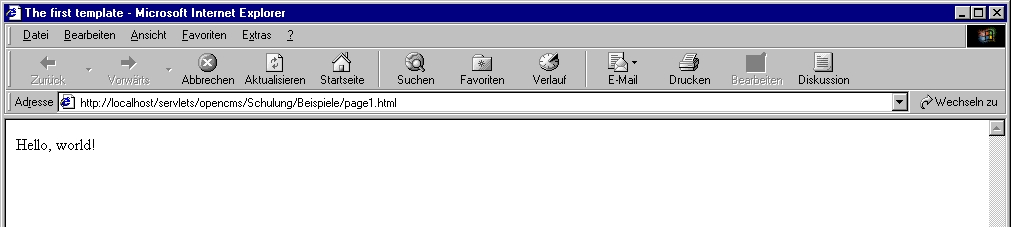
\includegraphics[width=\sgw]
                   {pics/templateMech/OutputHelloWorld}
\caption[The output of this example]
           {The output of this example}
\label{output}
\end{center}
\end{figure}



You can of course edit the body if you want to insert additional
text or pictures in the document. Data blocks can be used to
insert blocks of XML or HTML code in your document. The content of
these blocks can also be defined dynamically in Java classes. The
next example will show how this is done. Here the Text is directly
set into the datablock message within the template. But the text
can also be set by a Java method. In this case you should define
and include an dynamic element in your contenttemplate. The
controlling Java class has to be determied within the
elementdefinition. Change your contenttemplate to this:

%<?xml version="1.0"?>
<XMLTEMPLATE>
    <MESSAGE><![CDATA[Hello world!]]></MESSAGE>
    <TEMPLATE><![CDATA[
            ]]><ELEMENT name="dynamicelement"/><![CDATA[ <br>
        ]]><ELEMENT name="body"/>
    </TEMPLATE>

    <ELEMENTDEF name="dynamicelement">
        <CLASS>com.opencms.template.CmsXmlTemplate</CLASS>
        <TEMPLATE>/content/elements/element1</TEMPLATE>
    </ELEMENTDEF>
</XMLTEMPLATE>

\begin{verbatim}
<?xml version="1.0"?>
<XMLTEMPLATE>
    <MESSAGE><![CDATA[Hello world!]]></MESSAGE>
    <TEMPLATE><![CDATA[
        ]]><ELEMENT name="dynamicelement"/><![CDATA[ <br>
        ]]><ELEMENT name="body"/>
    </TEMPLATE>

    <ELEMENTDEF name="dynamicelement">
        <CLASS>CmsExample4</CLASS>
        <TEMPLATE>/content/elements/element1</TEMPLATE>
    </ELEMENTDEF>

</XMLTEMPLATE>
\end{verbatim}
\index{CLASS}
\index{ELEMENTDEF}

The elementdefinition (ELEMENTDEF) consist of three parts. The
name of the element. This is used to include it in the template
with the <ELEMENT> tag. The template file is the text file in the
element directory and the javaclass which process the template. In
this class tag we insert our new javaclass CmsExample4. If the
class is located inside a package, you have to type the fully
qualified class name inside the {\tag <CLASS>} tag.

Create the element1 in the folder {\dir /content/elements} with
this text:
\begin{xml}
<?xml version="1.0"?>\\
<XMLTEMPLATE>\\
<TEMPLATE>\\
\xtaba <PROCESS>greeting</PROCESS>\\
</TEMPLATE>\\
</XMLTEMPLATE>\\
\end{xml}

Then program your class like this:
%\input{examples/templateMechanism/datablocks/CmsExample3}
\begin{verbatim}
 import com.opencms.template.*;
import com.opencms.core.*;
import com.opencms.file.*;

public class CmsExample7 extends CmsXmlTemplate {


public byte[] getContent(CmsObject cms, String templateFile,
String elementName, Hashtable parameters, String templateSelector)
throws CmsException {

    CmsXmlTemplateFile template = getOwnTemplateFile(cms, templateFile, elementName, parameters, templateSelector);
    template.setData("greetings", "Hello from Java Class!");
    return startProcessing(cms, template, elementName, parameters, templateSelector);
    }
}
\end{verbatim}

This class sets in the datablock greeting the string "Hello from
Java Class".


\subsection{Using user-defined Methods}

Another way to insert dynamic content is to use user-defined
methods in the template. You have already seen how to use the {\it
getTitle()} method in a frametemplate in the second example. The
element template should contain the following text:

\begin{xml}
<?xml version="1.0"?>\\
<XMLTEMPLATE>\\
<TEMPLATE>\\
\xtaba <METHOD name="getHello"/>\\
</TEMPLATE>\\
</XMLTEMPLATE>\\
\end{xml}

This template contains the method tag . We will use a method that
returns the string {\name Hello, World from Java} and give it the
name {\meth getHello()}:

%\input{examples/templateMechanism/datablocks/CmsExample4}
\begin{verbatim}
 import com.opencms.template.*;
import com.opencms.core.*;
import com.opencms.file.*;

public class CmsExample4 extends CmsXmlTemplate {
    public Object getHello(CmsObject cms, String tagcontent, A_CmsXmlContent doc, Object userObject)
                         throws CmsException {
        return "Hello World from java!";
    }
}
\end{verbatim}

The output of the new template will be the same as that of the
previous example: it displays the string {\name Hello, World from
Java!} on the screen. The only difference is the procedure we
followed to accomplished the task of inserting something in the
document. In the previous example the process tag was replaced and
now we used the entirely new method {\name getHello()}.

\subsection{Details of OpenCms Template Programming}

\subsubsection{The relationship between Templates, Page Control Files, and Java Classes}

For every new page that is created with OpenCms, the system automatically creates a page
control file. This page control file determines the templates that are used by the new page
and the Java classes that are used to control them. Examples for page control files have already
been shown before. The different entries in these files will be explained in the following
section.
Below is the page control file for an earlier example:

\begin{xml}
<?xml version= "1.0 "?>\\
<page>\\
 <CLASS>com.opencms.template.CmsXmlTemplate</CLASS>\\
 <MASTERTEMPLATE>/content/templates/template5</MASTERTEMPLATE>\\
 <ELEMENTDEF name="body">\\
\xtaba  <CLASS>com.opencms.template.CmsXmlTemplate</CLASS>\\
\xtaba  <TEMPLATE>/content/bodys/page5.html</TEMPLATE>\\
 </ELEMENTDEF>\\
</page>\\
\end{xml}

As can be seen in the first line this file is an XML document.
There are two {\tag <CLASS>} entries and two entries for
templates. The first template entry is the one for the master
template and the second is for the body template. The name of the
master template file is enclosed between {\tag <MASTERTEMPLATE>}
tags. The <CLASS> tag above it determines the Java class that
controls the master template. This class is the generic {\name
com.opencms.template.CmsXmlTemplate} class and should always be
used to control the master template. The {\tag <ELEMENTDEF>} tag
defines an element with the name {\name body}. An element
definition must be provided for every subelement (subtemplate)
that is inserted in the document. The body element can be placed
in the contenttemplate with the element tag as follows: {\tag
<ELEMENT name="body"/>} You can place other subtemplates in your
document in the same way you placed the body template in it, by
inserting a {\tag <ELEMENT name="aNewName"/>} tag and element
definition in your document. The name for the new element can be
freely defined. The controlling Java class for the body template
can be one of the existing template classes or one that is derived
from these classes and defined by you. In the example above we
used the {\name CmsExample5} class, which defined the new method
{\meth getHello()}. \index{body element}

\subsubsection{The Difference between the Content and the Body Template}
The Contenttemplate is the template that holds the body template
and all of its subtemplates. The Frametemplate mainly defines the
layout of the whole page and the gaps in which the templates are
inserted. Figure~\ref{MasterEl2} shows the structure of a typical
web site created with OpenCms.

\begin{figure}[hbt]
\begin{center}
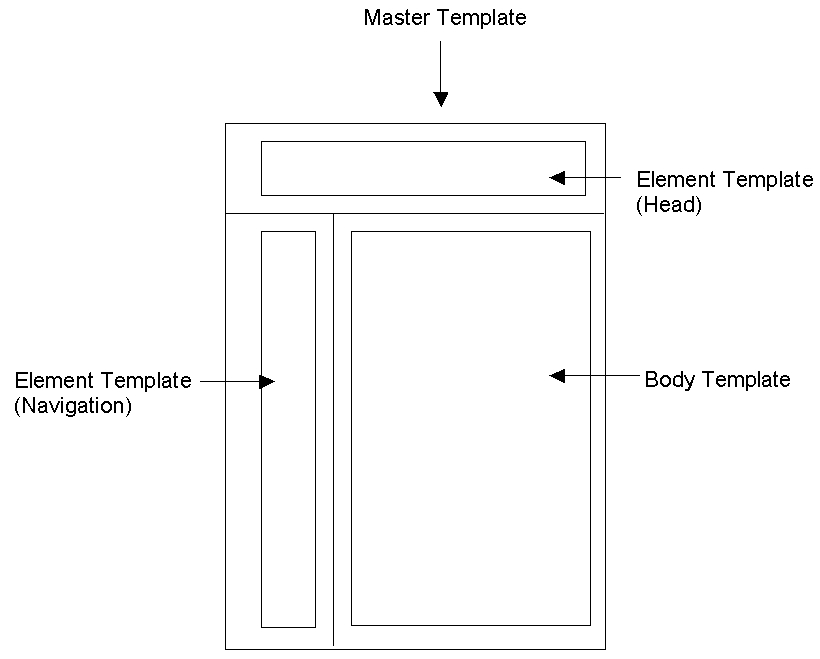
\includegraphics[width=\sgw]
                   {pics/templateMech/MasterAndElementes}
\caption[Master and Subelements]
           {Master and Subelements}
\label{MasterEl2}
\end{center}
\end{figure}

The frametemplate in this graphic contains a contenttemplate and
an element template (subtemplate) that creates the navigation. The
contenttemplate and all of the other element templates are also
capable of containing subtemplates. This enables you to structure
your document in any imaginable way. The frametemplate and the
contenttemplates can easily be reused for the design of other web
sites. \index{contenttemplate} \index{frametemplate} \index{body
template} \index{subtemplate}

\subsubsection{Process, Method and Element Tags}

The process, method and element tags enable you to insert dynamic
content in your web site. They have already been used in the first
examples. Their syntax and their usage will be discussed in the
following sections. The process tag can be used to insert the
content of data blocks in your document. The data blocks can be
defined in the document or set by Java classes. We will explain
how a process tag works by taking a look at a further example.
Here is the content of dynamic element template of this example:

\begin{xml}
<?xml version= "1.0 "?>\\
<XMLTEMPLATE>\\
<MESSAGE>\\
\xtaba <![CDATA[Hello, World ]]>\\
\xtaba <PROCESS>greeting</PROCESS>\\
</MESSAGE>\\

<TEMPLATE>\\
\xtaba <PROCESS>message</PROCESS>\\
</TEMPLATE>\\
</XMLTEMPLATE>\\
\end{xml}
\index{PROCESS}

There are two process tags in this template: the first inside the
data block {\name message} and the second inside the template tag.
The text inside the process tag defines the data block that will
be processed. In this example two data blocks will be processed,
one named {\name greeting} and one named {\name message}. The
{\name message} data block is defined in the template document.
The data block {\name greeting} is not defined in the document,
but set in the Java class that is associated with the template
(see the example above).

This way the data block can be set dynamically in the Java
classes. To show that it is possible to set the data block
randomly inside a Java class, the next examples insert a randomly
selected link to a web site. This is the content of the element
file:
\begin{xml}
<?xml version="1.0"?>\\
<XMLTEMPLATE>\\
<LINK1>www.opencms.com</LINK1>\\
<LINK2>www.yahoo.de</LINK2>\\
<TEMPLATE>\\
\xtaba  <![CDATA[\\
\xtaba  <a href="http://]]><PROCESS>link</PROCESS><![CDATA[">\\
\xtaba  Where will we go?</a>]]>\\
</TEMPLATE>\\
</XMLTEMPLATE>\\
\end{xml}

Here is the getContent method of the associated class:
\begin{verbatim}
public byte[] getContent(CmsObject cms, String templateFile,
String elementName, Hashtable parameters, String templateSelector)
throws CmsException {
    CmsXmlTemplateFile templateDocument = getOwnTemplateFile(cms, templateFile, elementName, parameters, templateSelector);
    String linkTarget;
    linkTarget = "link" + String.valueOf((int) (Math.random() * 2 + 1));
    templateDocument.setData("link", templateDocument.getDataValue(linkTarget));
    return startProcessing(cms, templateDocument, elementName, parameters, templateFile);
}
\end{verbatim}

The target of the link will be set randomly in a Java class.

The next example will show how to create tables or lists using the
process tag. You can use the process tag to set the data entries
in tables in Java classes. The table will be dynamically built in
the Java class by producing a string that concatenates the table
rows. The layout of the table is defined in the template. For this
example, we can use the template that was used in the previous
example: an empty site with a body element. The whole layout will
be defined in the element template. This is the content of the
element template:

\begin{xml}
<?xml version="1.0"?>\\
<XMLTEMPLATE>\\

<TEMPLATE>\\
\xtaba <![CDATA[ <H1>Animal list</H1>\\
\xtaba <table border=1>]]>\\
\xtaba <process>tablehead</process>\\
\xtaba <process>list</process>\\
\xtaba <![CDATA[\\
\xtaba </table>]]>\\
</TEMPLATE>\\
<tablehead>\\
\xtaba <![CDATA[\\
\xtaba <tr>\\
\xtaba <td>Nr</td>\\
\xtaba <td>animal</td>\\
\xtaba <td>owner</td>\\
\xtaba </tr>]]>\\
</tablehead>\\
<row>\\
\xtaba <![CDATA[\\
\xtaba <tr>\\
\xtaba <td>]]><process>number</process><![CDATA[</td>\\
\xtaba <td>]]><process>name</process><![CDATA[</td>\\
\xtaba <td> ]]><process>owner</process><![CDATA[</td>\\
\xtaba </tr>]]>\\
</row>\\
</XMLTEMPLATE>\\
\end{xml}

The template defines a table and two data blocks. The data block
{\name tablehead} defines a static heading for every column and
will be inserted in the table by the process tag. The content of
the table will be created in a Java class and will be set as the
data block {\name list.} The layout table's rows is defined by the
data block {\name row}. The Java class will set the content of
every row, concatenate the results and insert them in the document
as the data block {\name list}. Here again the getContent method:
\begin{verbatim}
public byte[] getContent(CmsObject cms, String templateFile,
String elementName, Hashtable parameters, String templateSelector)
throws CmsException {
    String[] owners = {"Martin", "Thomas", "Andreas", "Bill", "Michael", "Doris"};
    String[] animals = {"cat", "dog", "mouse", "rat", "bird", "snake"};
    CmsXmlTemplateFile template = getOwnTemplateFile(cms, templateFile, elementName, parameters, templateSelector);
    String list = "";
    for (int i = 0; i < animals.length; i++) {
        template.setData("number", i + "");
        template.setData("name", animals[i]);
        template.setData("owner", owners[i]);
        String row = template.getProcessedDataValue("row");
        list += row;
    }
    template.setData("list", list);
    return startProcessing(cms, template, elementName, parameters, templateSelector);
}
\end{verbatim}



The last example can be modified to produce a list instead of a table. The Java class can be
left unchanged and reused to create the list. This shows that it is possible to change the
layout in the template without having to change the Java class. This is the template that will
generate a list instead of a table:

\begin{xml}
<?xml version="1.0"?>\\
<XMLTEMPLATE>\\

<TEMPLATE>\\
\xtaba <![CDATA[ <H1>Animal list 2</H1>\\
\xtaba <ul>\\
\xtaba     ]]>\\
\xtaba     <process>list</process>\\
\xtaba     <![CDATA[\\
\xtaba </ul>]]>\\
</TEMPLATE>\\
<row>\\
\xtaba <![CDATA[\\
\xtaba <li>\\
\xtabb ]]><process>name</process><![CDATA[,\\
\xtabb ]]><process>owner</process><![CDATA[\\
\xtaba </li>]]>\\
</row>\\
</XMLTEMPLATE>\\
\end{xml}

The template places the data block {\name list} in an unsorted list. The rows' layout has been changed
to list entries. The name and the owner are set in the Java class and the list is generated in
the same way that it was in the last example. Note that the data block number is not used by the
template, but still set in the Java class. Although this is redundant, it is harmless because
the data block is set without being processed.

\subsubsection{The Method Tag}

The method tag is used to insert the output of a method in a document. You can use a new method
that is defined in a class that is derived from one of the existing template classes or a
standard method that is defined by the existing classes. In the last example of Chapter 2 we
created the new method {\name getHello()} to show how method tags are used.
In general, a method is used in a template by inserting a method tag. A method can take
parameters that are passed to the method by specifying them in the method tag.
\index{method tag}
The syntax for the method tag:
\begin{xml}
- <method name="test"/> \\
- <method name="test2">parameter(s)</method>\\
\end{xml}


The method tag can be used in two ways: for methods that don't need any parameters, the end tag
{\tag </method>} can be omitted and the tag can be closed by entering
{\tag />}. When parameters are passed
as a string to a method in the tag, the method tag has to be closed with the corresponding end
tag ({\tag </method>}).The examples that generated a table and a list using a process tag can
easily be
modified to use a method instead. The next example will show how to generate a table with the
new method {\meth getTable()}. Here is the body template:

\begin{xml}
<?xml version="1.0"?>\\
<XMLTEMPLATE>\\

<TEMPLATE>\\
\xtaba <![CDATA[ <H1>Animal list</H1>\\
\xtaba <table border=1>]]>\\
\xtaba <process>tablehead</process>\\
\xtaba <method name="getTable"/>\\
\xtaba <![CDATA[\\
\xtaba </table>]]>\\
</TEMPLATE>\\
<tablehead>\\
\xtaba <![CDATA[\\
\xtaba <tr>\\
\xtaba <td>Nr</td>\\
\xtaba <td>animal</td>\\
\xtaba <td>owner</td>\\
\xtaba </tr>]]>\\
</tablehead>\\
<row>\\
\xtaba <![CDATA[\\
\xtaba <tr>\\
\xtaba <td>]]><process>number</process><![CDATA[</td>\\
\xtaba <td>]]><process>name</process><![CDATA[</td>\\
\xtaba <td> ]]><process>owner</process><![CDATA[</td>\\
\xtaba </tr>]]>\\
</row>\\
</XMLTEMPLATE>\\
\end{xml}


The names of the owners and the animals have been changed to
emphasize that this table is not the same as the one that was
produced by using the process tag:

\begin{verbatim}
public class CmsExample9 extends CmsXmlTemplate {

public Object getTable(CmsObject cms, String tagcontent,
A_CmsXmlContent doc, Object userObject) throws CmsException {
    String[] owners = {"Elmar", "Randolf", "Sandra", "Geoffrey", "Claudia", "Doris"};
    String[] animals = {"spider", "eagle", "lion", "cheetah", "scorpion", "snake"};
    CmsXmlTemplateFile template = (CmsXmlTemplateFile) doc;
    String list = "";
    for (int i = 0; i < animals.length; i++) {
        template.setData("number", i + "");
        template.setData("name", animals[i]);
        template.setData("owner", owners[i]);
        String row = template.getProcessedDataValue("row");
        list += row;
    }
    return list;
}
}
\end{verbatim}

\subsubsection{Element Tag and Element Definition}

The element tag is used to insert subelements (subtemplates) in a web site. The element
definition defines the template and Java class that are used for the element. Examples of
element definitions were shown in an earlier section. In this section, we will take a look at the
element tag and element definition. The element tag must have the following syntax:
\begin{xml}
<ELEMENT name="aName"/>
\end{xml}


where aName must be replaced with the name of the element. A valid element definition has the
following structure:
\begin{xml}
<ELEMENTDEF name="aName">\\
\xtaba <TEMPLATE>nameOfTheTemplateFile</TEMPLATE>\\
\xtaba <CLASS>nameOfTheControllingClass</CLASS>\\
\xtaba <PARAMETER name="param1">value1</PARAMETER>\\
\xtaba <PARAMETER name="param2">value2</PARAMETER>\\
</ELEMENTDEF>\\
\end{xml}
\index{ELEMENTDEF}

In the element definition, the template file and the controlling
Java class are specified in the template and the class tag. It is
also possible to pass parameters to the controlling Java class.
Parameters that are specified in the element definition are
accessible in the Java class. They are stored in a hash table
together with the parameters that are appended to a URL. The
element definition is defined either in the document in which the
element is inserted, or in the page control file. The element
definition can also be overridden in the page control file. If an
element definition is specified in both the file in which the
element is inserted and in the page control file, the element
definition stored in the page control file takes precedence. This
means that the page control file can be used to modify a default
element definition. The next example will show the effect of
overriding element definitions. First we need to create a template
that contains elements that consist of templates using data from
the previous examples. This is the frametemplate for the new page:
\begin{xml}

<?xml version="1.0"?>\\
<XMLTEMPLATE>\\
<TEMPLATE>\\
<![CDATA[\\
<HTML>\\
<HEAD>\\
\xtaba <TITLE>]]><method name="getTitle"/><![CDATA[</TITLE>\\
</HEAD>\\
<BODY>\\
\xtaba <TABLE border width="100\%" height="100\%">\\
\xtaba   <TR height="30\%">\\
\xtaba           <TD width="20\%"><IMAGE src="\\
\xtaba ]]><method name="getServletPath"/><![CDATA[\\
\xtaba pics/opencmslogo.gif" align="center">\\
\xtaba </TD>\\
\xtaba           <TD width="80\%" align="center">\\
\xtaba ]]><element name="hello"/><![CDATA[\\
\xtaba </TD>     \\
\xtaba   </TR>\\
\xtaba   <TR height="70\%">\\
\xtaba           <TD width="20\%" align="center" valign="top">\\
\xtaba                   ]]><element name="random"/><![CDATA[\\
\xtaba           </TD>\\
\xtaba           <TD width="80\%" align="center">\\
\xtaba                   ]]><element name="contenttemplate"/><![CDATA[\\
\xtaba           </TD>\\
\xtaba   </TR>\\
\xtaba </TABLE>\\
</BODY>\\
</HTML>]]>\\
</TEMPLATE>\\

<ELEMENTDEF name="hello">\\
\xtaba <TEMPLATE>/content/elements/element1</TEMPLATE>\\
\xtaba <CLASS>CmsExample4</CLASS>\\
</ELEMENTDEF>\\

<ELEMENTDEF name="random">\\
\xtaba <TEMPLATE>/content/elements/element2.html</TEMPLATE>\\
\xtaba <CLASS>CmsExample6</CLASS>\\
</ELEMENTDEF>\\

</XMLTEMPLATE>\\
\end{xml}
\index{ELEMENTDEF} The template defines a table with two rows and
two columns. A picture of the  OpenCms logo is placed in the first
row of the first column. An element called {\name hello} is placed
in the second column of the first row. The corresponding element
definition specifies this element as the one we used before: it
displays the string {\name Hello, World from Java!} on the screen.
The second row in the first column contains an element called
{\name random}. This element is the random link that we created
before. The contentelement is inserted in the second column of row
2. This is the content of the element included in the
contenttemplate:

\begin{xml}
<?xml version="1.0"?>\\
<XMLTEMPLATE>\\
<TEMPLATE>\\
\xtaba <![CDATA[\\
\xtaba <TABLE border>\\
\xtaba   <TR>\\
\xtaba <TD valign="top">\\
\xtaba ]]><element name="animaltable"/><![CDATA[\\
\xtaba </TD>\\
\xtaba           <TD valign="top">\\
\xtaba ]]><elementname="animallist"/><![CDATA[\\
\xtaba </TD>\\
\xtaba   </TR>\\
\xtaba </TABLE>]]>\\
</TEMPLATE>\\
<ELEMENTDEF name="animaltable">\\
\xtaba <TEMPLATE>/content/elements/element7.html</TEMPLATE>\\
\xtaba <CLASS>CmsExample7</CLASS>\\
</ELEMENTDEF>\\

<ELEMENTDEF name="animallist">\\
\xtaba <TEMPLATE>/content/elements/element8.html</TEMPLATE>\\
\xtaba <CLASS>CmsExample7</CLASS>\\
</ELEMENTDEF>\\

</XMLTEMPLATE>\\
\end{xml}


The template defines a table with two elements that contain data
from previous examples: the table and a list of the animals and
their owners. When you look at the page you will see that the
elements are all placed in the document in the positions that are
defined in the template. The effect of overriding an element
definition will be shown in the next example. An element
definition is overridden by adding another element definition in
the page control file. This is the content of the original page
control file:
\begin{xml}
<?xml version= "1.0 " encoding= "ISO-8859-1 "?>\\
<page>\\
 <CLASS>com.opencms.template.CmsXmlTemplate</CLASS>\\
 <MASTERTEMPLATE>/content/templates/template8</MASTERTEMPLATE>\\
 <ELEMENTDEF name="body">\\
\xtaba  <CLASS>com.opencms.template.CmsXmlTemplate</CLASS>\\
\xtaba  <TEMPLATE>/content/bodys/page\_11.html</TEMPLATE>\\
 </ELEMENTDEF>\\
</page>\\
\end{xml}


To change the content of the {\name hello} element you can add a definition for the
{\name hello} element to the page control file:
\begin{xml}
<?xml version= "1.0 " encoding= "ISO-8859-1 "?>\\
<page>\\
 <CLASS>com.opencms.template.CmsXmlTemplate</CLASS>\\
 <MASTERTEMPLATE>/content/templates/template8</MASTERTEMPLATE>\\
 <ELEMENTDEF name="body">\\
\xtaba  <CLASS>com.opencms.template.CmsXmlTemplate</CLASS>\\
\xtaba  <TEMPLATE>/content/bodys/page\_12.html</TEMPLATE>\\
 </ELEMENTDEF>\\
 <ELEMENTDEF name="hello">\\
\xtaba  <TEMPLATE>/content/elements/element2.html</TEMPLATE>\\
\xtaba  <CLASS>CmsExample6</CLASS>\\
 </ELEMENTDEF>\\

</page>\\
\end{xml}


Because this element definition will be used instead of the one
that is defined in the template, the random link (element template
of example 6) will be displayed instead of the {\name Hello, World
from Java!} text (see example 12). For missing parts of the
element definition the element definition for the body element in
the page control file is used. If the element's class or template
is not specified, it will be taken from the body element
definition in the page control file. You can see this by deleting
the definition for the {\name hello} element in the master
template. Doing this will display the content of the body element
instead of the {\name Hello, World from Java!} text (see example
13). Example 14 will show how parameters that are specified in an
element definition are used. Example 13 has been modified and
parameters added to the definition of the element {\name hello.}
The Java class and the element's template have been modified to
insert the parameters. The parameters are used to specify the
element's foreground and background colors. This is the new
definition of the {\name hello} element:
\begin{xml}
<ELEMENTDEF name="hello">\\
\xtaba <TEMPLATE>/content/elemetns/page\_14\_param.html</TEMPLATE>\\
\xtaba <CLASS>CmsExample14</CLASS>\\
\xtaba <PARAMETER name="foreground">blue</PARAMETER>\\
\xtaba <PARAMETER name="background">green</PARAMETER>\\
</ELEMENTDEF> \\
\end{xml}
\index{PARAMETER}

This element definition is located in the frametemplate. Two
parameters, {\name foreground} and  {\name background}, define the
colors of the element. These colors are defined in the Java class
that controls the element's template.


\subsubsection{Standard Methods of the OpenCms Template Mechanism}

The {\name com.opencms.template.CmsXmlTemplate} class defines a number of basic methods that can
be used when creating a template. The following section describes the functionality they provide
and how it is used.

The following table describes the standard methods that are defined in the
{\name CmsXmlTemplate} class:

\begin{center}
\begin{table}\footnotesize
\begin{tabular}{|l|p{0.73\linewidth}|}
\hline
Method  & Description\\
\hline
\index{getTitle()} getTitle() &
Is used to refer to the title of a page in a template. The title, defined as a
property of a page when it is being created, can easily be changed by selecting Properties from
the context menu of the page's file.\\
\index{getRequestIp()} getRequestIp() &
Returns the IP address of the machine that requested a page.\\
\index{getSessionId()} getSessionId() &
Provides a means of receiving an identification number that is used to identify
a special user. Session Ids are defined by using cookies. Cookies are short text files that are
stored on the client and can be used to identify users and keep track of their actions.\\
\index{getServletPath()} getServletPath() &
Returns the relative path of the directory in which the servlets reside
on the server. This method is used to write templates that are independent of the servlet path.
The servlet path can be changed without affecting the template files when this method is used to
refer to the path.\\
\index{getPathUri()} getPathUri() &   Returns the path of the requested file.\\
\index{getFileUri()} getFileUri() &   Returns the file name of the requested file.\\
\index{getStyleSheet()} getStyleSheet() &
Is useful for inserting the appropriate style sheet definition for different
browsers in a template. Two data blocks with the predefined names <stylesheet-ie> and
<stylesheet-ns> have to be used in the template to specify the name of the style sheet files
for the browser. The getStyleSheet method returns the path to the appropriate style sheet based
on the browser that is used by the client. By using this method and different style sheets for
Netscape Navigator and Windows Explorer, the appropriate style sheet is used if the method
manages to detect the user's browser.\\
\index{getQueryString()} getQueryString() &
Returns a string that contains the parameters that have been passed
with the URL when the page was requested.\\
\index{getFrameQueryString()} getFrameQueryString() &
Provides access to the parameters that have been passed with the URL
in a frame. In general, the parameters are only accessible in the file that was requested and
contains the frames. Each frame usually contains a different HTML page. The parameters that are
passed to the parent file are not directly accessible in the frames.\\
\index{parameters()} parameters() &
Is used for debugging. It returns all of the parameters for the current template
file that are passed with the URL. It also returns additional parameters for internal use that
contain the name of the element, the complete file name of the body element, and the controlling
Java class for this element.\\
\index{getFrameTarget()} getFrameTarget() &
Is used to specify the target for a link in a template that works both
in a version with and without frames. The parameter cmsframe is passed with the URL and used to
select the version that does not use frames by setting it to {\name plain}. If cmsframe is passed as
the parameter and is equal to {\name plain}, the target will be set to the empty string, meaning that
the method returns {\name target=""}. If cmsframe is not passed as the parameter with the URL, the
method returns the string {\name  target="tagcontent"}. The tagcontent is the parameter that
is passed
to  the method by defining it in the method tag. If the  tagcontent parameter is not passed,
the method returns {\name target="\_top"} for the frames version. This is a syntax example for the
method:
{\tag <method name="getFrameTarget">main</method>}
In this case the method returns the string:
{\name target="main"} if the frame version is used, and {\name target=""} for the version
that does not use
frames. Note: this method is only useful if you are creating both a frames and a non-frames
version of a web site.\\ \hline
\end{tabular}
\caption[Standard methods]{Standard methods}
\label{StaMe}
\end{table}
\end{center}

\section{Multiple templates in one XML-file}
%============================================================================
\subsection{Multiple content-areas in one content template}

You already noticed that the entry-point of every page is the page
control file. From there, the combination of frame and
contenttemplate  is chosen and in the contenttemplate the
content-area (the one body element) is inserted. Every other
element which is inserted and defined in the content or
frametemplate is kind of static and is shown on every page which
uses this template. But what if someone wants that the dynamic
content of his page is not shown in one single block, but in
several blocks which might be separated by advertising banners or
something like that? OpenCms provides a way to handle this.
Multiple templates (content areas) can be defined within one XML
file (in this case the body file in the {\dir content/bodys}
directory). Each template can be given a different name.
\begin{xml}
<TEMPLATE>\\
...\\
</TEMPLATE>\\
<TEMPLATE name="body">\\
...\\
</TEMPLATE>\\
<TEMPLATE name="body1">\\
...\\
</TEMPLATE>\\
\end{xml}


The default template doesn't need a name.  Now we have two
templates, which both have to be inserted in content template.
This can be done by an element definition in the content template:
\begin{xml}
<ELEMENTDEF name="elementName">\\
  <TEMPLATESELECTOR>aName</TEMPLATESELECTOR>\\
</ELEMENTDEF>\\
\end{xml}
\index{TEMPLATESELECTOR}

The trick is that this elementdefinition neither specifies an XML file (with the
{\tag <template>} tag),
 nor a controlling java class. If both are not determined, OpenCms uses the file and the class
from the body element in the page control file. The
templateselector tells that in this case the second template has
to be chosen and displayed.  If a template selector is not
defined, the default template will be displayed (the template
without a name). This selection can be overridden in the Java
class that controls the template file.

You can also use the WYSIWYG-Editor to create an OpenCms-generated
body file that contains multiple templates Figure~\ref{NewBody}.

\begin{figure}[hbt]
\begin{center}
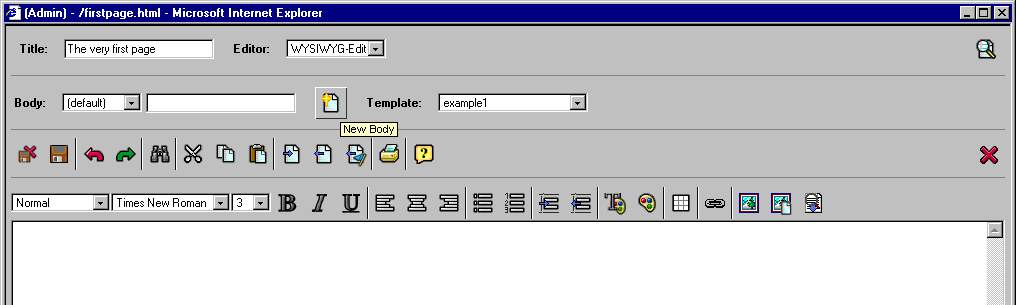
\includegraphics[width=\sgw]
                   {pics/templateMech/NewBody}
\caption[Creating a new body with the Editor]
           {Creating a new body with the Editor}
\label{NewBody}
\end{center}
\end{figure}

All you have to do is click on the new body icon and a template
with the name {\it body1} ({\name body2} for the next and so
on...) is inserted in the template file. You can change the name
after you have finished creating the new template. Afterwards, you
can edit your content template and insert the further templates.
Here is complete sourcecode for a contenttemplate that inserts the
elements {\name body} and {\name second} which both are stored in
the same file:

\begin{xml}
<?xml version="1.0"?>\\
<XMLTEMPLATE>\\
<TEMPLATE>\\
<![CDATA[\\
\xtaba <TABLE border width="100\%" height="100\%">\\
\xtaba   <TR height="30\%">\\
\xtabb             <TH colspan=3 width="100\%" align="center"> \\
\xtabb The Head section </TH> \\
\xtaba   </TR>\\
\xtaba   <TR height="70\%">\\
\xtabb <TD width="20\%" align="center" valign="top">\\
\xtabb  Navigation </TD>\\
\xtabb             <TD width="40\%" align="center">]]>\\
\xtabb <element name="body"/><![CDATA[\\
\xtabb </TD>\\
\xtabb             <TD width="40\%" align="center">]]> \\
\xtabb <element name="second"/><![CDATA[\\
\xtabb </TD>\\
\xtaba   </TR>\\
\xtaba </TABLE>\\
</TEMPLATE>\\

<ELEMENTDEF name="second">\\
\xtaba   <TEMPLATESELECTOR>body1</TEMPLATESELECTOR>\\
</ELEMENTDEF>\\

</XMLTEMPLATE>\\
\end{xml}

This contenttemplate inserts two elements into two independent
cells of a table. After creating a template like that, you can
create a page that uses a template containing this
contenttemplate. Then create a second body with the
WYSIWYG-editor, and insert content in the two bodys. The body can
be chosen in the body-list in the head section of the
WYSIWYG-editor. The page control does not have to be changed.
Afterwards, the output could look like Figure~\ref{2Bodies}.

\begin{figure}[hbt]
\begin{center}
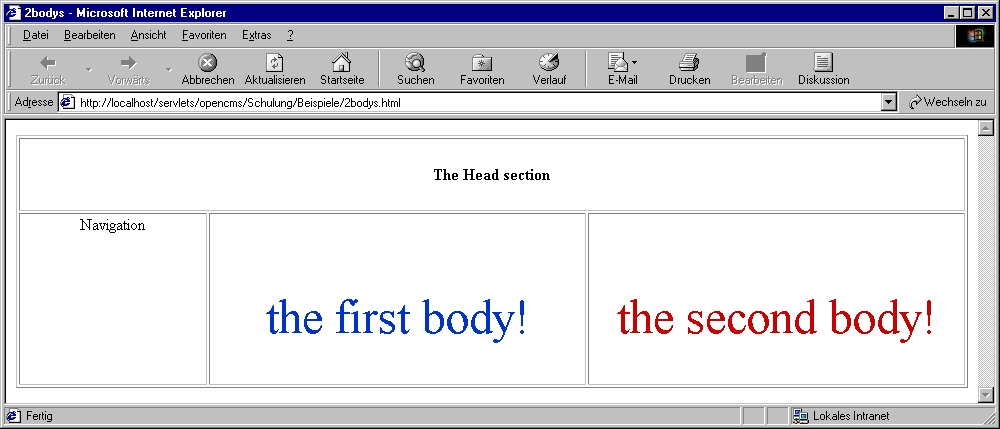
\includegraphics[width=\sgw]
                   {pics/templateMech/2Bodies}
\caption[2 Bodies]
           {2 Bodies}
\label{2Bodies}
\end{center}
\end{figure}

The way of processing is now the following: The template mechanism
processes the content template and comes to the body element. It
is known from the page control file where this element can be
found. Because no special templateselector is specified, the
default one is used. After that, the template mechanism comes to
the element second. Because nothing else is specified, the
template mechanism knows to look in the file which was used
before. But now a template selector is specified, and not the
default, and because of this the second template {\name body1} is
inserted. It is important to realize that of course every page
that wants to use this content template now has to define a second
template with the name {\name body1}.

\subsection{Dynamic insertion of templates}

The templateselector can be used to change the templates dynamically as well. In this case the
different templates, which are still stored together in one XML-file, are not displayed at the
same time, but one after another.
This functionality can of course be realized without the templateselector, by simply creating
different pages (XML-files that use the same master), but if the pages logically belong together,
 it is usefull to do it this way.
The best example is the creation of forms. Forms normally have more than one page, at least one
to insert the data and one page to confirm the input or even show error messages. It is quite
easy to store these templates in one XML-file and choose the right one with the templateselector.
  Of course it is not possible to realize this functionality only from the interface site. The
template selector has to be set inside a Java class in this case.
To provide the functionality from  the interface site only the different bodys have to be
prepared. This has to be known when forms are required. The usage and customization of forms
will be shown in one of the following chapters.

\subsection{Forms}
\index{forms}
HTML forms are used to add functionality to a web site. With HTML forms, you can receive feedback
 from the surfers or enable them to order products, product-related materials, or anything else
you'd like to make available.
The input that is received from the user can be evaluated in a number of ways. Traditionally,
this is done by a cgi program that processes the data on the server. Major drawbacks of this
approach are the inefficiency and the security holes. When using cgi programs to process the
data, every request to the cgi program creates a new process, which produces a significant load
on the operating system. The cgi approach does not come with a security model that prevents
incorrect cgi programs from crashing the server.
These disadvantages have been overcome by Java servlets, which provide a way to write efficient,
platform independent, and secure server-applications. Servlets are special Java classes that can
be executed by a server that supports the Java servlet API. Servlets take advantage of the built
in security model and the platform independence of the Java language. An instance of a servlet
is loaded either when the server is started (this can be specified by in the server's Services)
or when the servlet is first accessed. Concurrent requests to one servlet are handled by
multiple threads of the servlet. After a servlet is first loaded and initialized, it is
generally not unloaded until the server shuts down. This ensures the servlet class is loaded
and initialized once when the servlet is accessed for the first time.
OpenCms itself is a servlet that enables the evaluation of HTML forms writing customized Java
classes. Although not servlets themselves, these classes have the same advantages as servlets:
they are efficient, portable, and secure!

\subsubsection{A first example using forms}
\index{hidden input field}
Because the form shouldn't be evaluated when it is requested for the first time, a little trick
can help to detect if the page is being displayed for the first time or if it has already been
filled out. A hidden input field in the form acts as a flag that indicates if the input fields
have to be checked or not. A hidden input field works similar to a cookie, except that cookies
are sent for every request and not just in response to a form posting. The value of this hidden
field is set in the Java class. When the page is first requested, the value of the field is not
defined. The Java class detects this and omits checking the input fields. This is the section
with the hidden input field:

\begin{xml}
<FORM>... \\
<INPUT type="hidden" name="action" \\
value="]]><process>setaction</process><![CDATA[">\\
...</FORM>\\
\end{xml}

\begin{figure}[htb]
\begin{minipage}[t]{0.499\linewidth}
  \begin{center}
  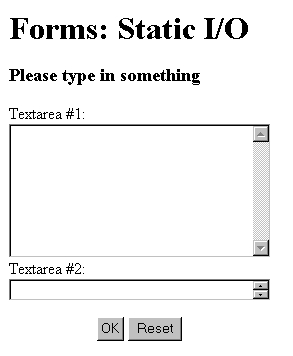
\includegraphics[clip,width=\sgw]
                   {pics/templateMech/StaticIO1}
 \end{center}
\end{minipage}
\hfill
\begin{minipage}[t]{0.499\linewidth}
   \begin{center}
   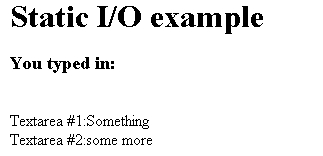
\includegraphics[clip,width=\sgw]
                   {pics/templateMech/StaticIO2}
   \end{center}
\end{minipage}
\caption[(Using forms]
           {Using forms}
 \label{forms}
\end{figure}

Figure~\ref{forms} shows the two pages of the template.
The first consists of two different input
fields in which free text can be entered:
After typing in the text, you can click on the OK or the Reset button. These two are the
standard buttons that are used with HTML forms. Clicking on one of these buttons sends the form
data.

\begin{xml}
<INPUT type=submit value="OK">\\
<INPUT type=reset value="Reset">\\
\end{xml}
\index{INPUT}

The Reset button automatically erases the input field without sending the data. Clicking on the
OK button displays the text in the input fields on the second page of the template. The form tag
determines the method that is used to send the data to the server. The controlling Java class
selects the appropriate template by setting the template selector with the name of the template
section.
The result on the confirmation page after clicking on the OK button is shown in
Figure~\ref{forms} on the right side.

As you can see, the confirmation page shows the user his/her input again so that he/she can see
what was sent to the server. The confirmation page is selected in the Java class by setting the
template selector. Assuming you have named the confirmation template {\name reply}, all you have
to do to tell OpenCms that this template should be used to create the web page that is shown to
the user, is to set the template selector in your class:

{\code templateSelector="reply"; }

\subsubsection{Presetting values}

In order to use preset values, the controlling Java class has to set the values of the fields
with a preset value or with the input the user has already given. This can be accomplished by
setting the value of a field via the process tag:

\begin{xml}
<TEXTAREA cols=30 rows=8 name=comment>\\
]]><process>comment</process><![CDATA[\\
</TEXTAREA>\\
\end{xml}


The value of the input field will be the value of the data block comment. This data block is
specified in the template as an empty data block: If you did not initialize the data block,
you will get an error message that the data block is unknown. You should always define the
value  as an empty element in the beginning of the body template:

\begin{xml}
<XMLTEMPLATE>...\\
<comment></comment> ... \\
<TEMPLATE>...\\
\end{xml}


A value is preset by entering text. When the template is first started, the data block is set
with this value:
\begin{xml}
<XMLTEMPLATE>...\\
<comment>Please fill in something here!</comment>...\\
<TEMPLATE>...\\
\end{xml}


Of course it is more flexible to preset the values in a Java Method. This way it is possible to
preset an imput field with the name of the current user or the actual date for example.




\section{Frames}
%============================================================================
\subsection{Framsets in OpenCms}
 \index{frames}
The usage of frames is quite easy with OpenCms. One big difference
to the usage of frames in standard HTML is that in OpenCms,
everything is stored together in one file.  In this part, we will
create a simple page with two frames to show the basic structure.
The frameset and the inserted parts (templates) are defined in the
frametemplate. The complete code for a frametemplate with 2 frames
is shown here:
\begin{xml}
<?xml version="1.0"?>\\
<XMLTEMPLATE>\\

<TEMPLATE><![CDATA[\\
<!DOCTYPE HTML PUBLIC "-//W3C//DTD HTML 4.0 Transitional//EN">\\
<HTML>\\
  <HEAD><TITLE>Seite mit Frames</TITLE></HEAD>\\
  <FRAMESET ROWS="100,*">\\
\xtaba     <FRAME NAME="frame\_head" src="]]>\\
\xtabb <METHOD name="getUri"/>\\
\xtabb            <METHOD name="getFrameQueryString">temp\_head</METHOD>\\
\xtabb            <![CDATA[">\\
\xtaba     <FRAME NAME="frame\_body" src="]]>\\
\xtabb            <METHOD name="getUri"/>\\
\xtabb            <METHOD name="getFrameQueryString">temp\_body</METHOD>\\
\xtabb            <![CDATA[">\\
  </FRAMESET>\\
</HTML>]]>\\
</TEMPLATE>\\
\index{getFrameQueryString}
<TEMPLATE name="temp\_head"><![CDATA[\\
\xtaba <!DOCTYPE HTML PUBLIC "-//W3C//DTD HTML 4.0 Transitional//EN">\\
\xtaba <HTML>\\
\xtaba   <HEAD><TITLE>Seite mit Frames</TITLE></HEAD>\\
\xtaba   <BODY>\\
\xtabb             <P ALIGN="center">\\
\xtabb       ]]><ELEMENT name="nav\_head"/><![CDATA[\\
\xtabb     </P>\\
\xtaba   </BODY>\\
\xtaba </HTML>]]>\\
</TEMPLATE>\\

<TEMPLATE name="temp\_body"><![CDATA[\\
\xtaba <!DOCTYPE HTML PUBLIC "-//W3C//DTD HTML 4.0 Transitional//EN">\\
\xtaba <HTML>\\
\xtaba   <HEAD><TITLE>Seite mit Frames</TITLE></HEAD>\\
\xtaba   <BODY>\\
\xtabb     <P ALIGN="center">\\
\xtabb       ]]><ELEMENT name="contenttemplate"/><![CDATA[\\
\xtabb     </P>\\
\xtaba   </BODY>\\
\xtaba </HTML>]]>\\
</TEMPLATE>\\

<ELEMENTDEF name="nav\_head">\\
\xtaba <CLASS>com.opencms.defaults.CmsXmlNav</CLASS>\\
\xtaba <TEMPLATE>/content/elements/nav\_head</TEMPLATE> \\
</ELEMENTDEF>\\

</XMLTEMPLATE>\\
\end{xml}


The frameset is here defined within the default template (the one
without a name) with the normal {\tag <FRAMESET>}-tag.  The
difference to the standard HTML way is now that is has to be
determined what template has to be inserted. This is done by the
method {\meth getFrameQueryString()}. The method gets the name of
the template that should be inserted as a parameter. The right
template is then choosen by the templateselector. The mechanism
evaluates the parameter {\name cmsframe},  which is returned from
the method {\meth getFrameQueryString()}. It would be possible to
simply add the parameter by hand ( {\tag <![CDATA[
?cmsframe=temp\_head} ), but this would cause problems if further
parameters are appended from somewhere. The method {\meth
getFrameQueryString()} solves this problem and handles further
parameters. Thus it is recommended to use the method always.
\index{cmsframe} The method {\meth getUri()} returns the URI
including the filename of the actual file. The templates which
have to be inserted in the frames are defined afterwards. The
certain elements that should be inserted are specified within the
templates. Here are two elements inserted, one for the navigation
(nav\_head) and one content element. Of course, there has to be an
elementdefinition for the navigation element at the end of the
XML-file.  The navigation template for this example looks like
this:

\begin{xml}
<?xml version="1.0"?>\\
<XMLTEMPLATE>\\

<NAVENTRY><![CDATA[\\
\xtaba   <A HREF="]]>\\
\xtaba   <PROCESS>navlink</PROCESS>\\
\xtaba     <METHOD name="getFrameQueryString">temp\_body</METHOD>\\
\xtaba     <![CDATA[" ]]>\\
\xtaba     <METHOD name="getFrameTarget">frame\_body</METHOD>\\
\xtaba     <![CDATA[>]]>\\
\xtaba   <PROCESS>navtext</PROCESS><![CDATA[\\
\xtaba   </A>]]>\\
</NAVENTRY>\\

<TEMPLATE>\\
\xtaba   <![CDATA[<TABLE BORDER=1 CELLPADDING=2 CELLSPACING=0><TR><TD>]]>\\
\xtaba   <METHOD name="getNavRoot">1</METHOD>\\
\xtaba   <![CDATA[</TD></TR></TABLE>]]>\\
</TEMPLATE>\\

</XMLTEMPLATE>\\
\end{xml}
\index{getNavRoot}
\index{getFrameTarget}

A reference to a page that should be displayed in another frame in standard HTML looks like
this:

{\tag <a href="aName.htm" target="aFrame">aNavText</a>}

The parameter {\name aFrame} determines the frame in which the source should should be displayed,
and the parameter {\name aName.htm} determines the source that should be inserted.
Here the parameter {\name aName.htm} has to be expanded by  a parameter that defines what template has
to be selected to insert. This is again done by the templateselector, and the parameter
({\name cmsframe}) is again inserted by the method {\meth getFrameQueryString()} to allow further
parameters.

\begin{xml}
<A HREF="]]>\\
  <PROCESS>navlink</PROCESS>\\
    <METHOD name="getFrameQueryString">temp\_body</METHOD>\\
    <![CDATA[" ]]>\\
    <METHOD name="getFrameTarget">frame\_body</METHOD>\\
    <![CDATA[>]]>\\
  <PROCESS>navtext</PROCESS><![CDATA[\\
</A>]]>\\
\end{xml}


The parameter {\name target} is here inserted by the method {\meth getFrameTarget()}. Again, this is
the recommended way. Of course, the parameter could be simply added by inserting
{\tag target="frame\_body"}, but you will see in the next paragraph why the usage of the method
has
advantages.
To understand the difference, here the above code block is now shown without the usage of
methods:
\begin{xml}
<A HREF="]]>\\
  <PROCESS>navlink</PROCESS>\\
    <!CDATA[?cmsframe="temp\_body" TARGET="frame\_body">]]>\\
  <PROCESS>navtext</PROCESS><![CDATA[\\
</A>]]>\\
\end{xml}


Maybe this helps to understand which text is inserted by the methods. But again, it is allways
recommended to make usage of these methods, to write templates that can be easily reused and
provide full functionality! Unfortunately it has to be mentioned here that some older versions
of OpenCms can�t handle the usage of these methods together with the class {\it CmsXmlNav}.
You will get an error message in this case.

Pages which are inserted into the frames can now easily be created. You only have to choose the
above master template. The output for three inserted pages could for example look like
~\ref{frames1}.

\begin{figure}[hbt]
\begin{center}
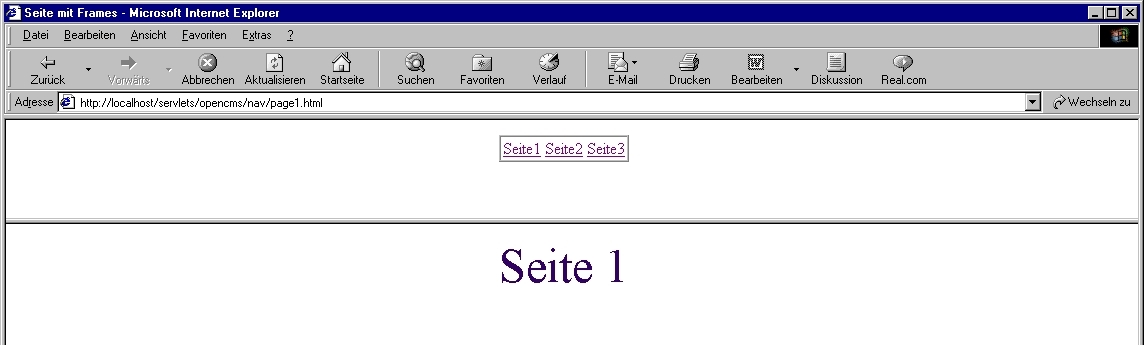
\includegraphics[width=\sgw]
                   {pics/templateMech/frames_kurz}
\caption[A page with frames]
           {A page with frames}
\label{frames1}
\end{center}
\end{figure}

\subsection{Frames- and non-frames-versions}

Often a web site has to be build in two versions, one with frames,
and one without frames. This way users with older browsers are
able to visit the site as well. These two versions can be achieved
with one frametemplate in OpenCms. All you have to do is to extend
the frame template by one further template. This template should
be named {\name plain}. It defines the layout for the site without
frames. The other templates that are already defined are inserted
in the {\name plain}-template as well. One implementation of the
{\name plain}-template is shown now:

\begin{xml}
<?xml version="1.0"?>\\
...\\
<TEMPLATE name="plain"><![CDATA[\\
<HTML> \\
<HEAD>\\
\xtaba <TITLE>]]><method name="getTitle"/><![CDATA[</TITLE>\\
</HEAD>\\
<BODY>\\
\xtaba <TABLE border width="100\%" height="100\%">\\
\xtaba   <TR height="30\%">\\
\xtabb             <TD align="center">]]> \\
\xtabb              <element name="nav\_head"/> <![CDATA[</TD>\\
\xtaba   </TR>\\
\xtaba   <TR height="70\%">\\
\xtabb             <TD align="center">]]>\\
\xtabb              <element name="body"/> <![CDATA[</TD>\\
\xtaba   </TR>\\
\xtaba </TABLE>\\
</BODY>\\
</HTML>]]>\\
</TEMPLATE>\\

<ELEMENTDEF name="nav\_head">\\
...\\
</XMLTEMPLATE>\\
\end{xml}

This template inserts exactly the same subtemplates as the one that uses frames. Even the
template for the navigation is the same. The are only set inside a table instead of frames.
Now it becomes usefull that we implemented the navigation with the {\meth getFrameTarget()}
 method.
The navigation would not work with a table, if the parameter {\tag target=...} had
simply be added. The {\meth getFrameTarget()} method distinguishes between the frames and
the non frames version an drops
the parameter {\name target} if necessary. If you implemented the templates like this, a simple call
to the URL of a page that uses this master would start the frames version, which is defined in
the default template. You can choose the non-frames version by add the parameter
{\name ?cmsframe=plain}
to the URL. The output would then look like Figure~\ref{noFrames}.

\begin{figure}[hbt]
\begin{center}
\includegraphics[width=\sgw]
                   {pics/templateMech/frames_2}
\caption[A version without frames]
           {A version without frames}
\label{noFrames}
\end{center}
\end{figure}


\section{Modules}
%============================================================================
\subsection{What is a module?}
\index{module mechanism}
OpenCms provides a module mechanism to add further functionality to the system. A module is a
dynamic extension of the system with XML templates and Java classes. A module can be uploaded,
installed and uninstalled from within the system. An example of a module is the back office part
of a discussion forum on a web site that was created with OpenCms. You might wish to administer
the forums and comments from within OpenCms, i.e. delete or create databa se entries in a
specific, possibly external, databa se. You would include your pages with the dialogs and the
classes that implement this functionality in the module. A module can but does not have to
include Java classes, templates and documentation.

A module is a zip file that contains a number of other files (specified in detail below). This
module/zip file can be uploaded using the OpenCms view {\name Administration}. You can upload the
file from your local machine to the server through the OpenCms system or via ftp, and then specify
the path to the zip file in the dialog. The zip file will then be unpacked and it's content will
be copied to the specified location in the virtual file system. Information about these
locations as well as other information about the module is stored in the system's registry,
which makes it possible to uninstall it. After the copy is finished, an event handler method
of one of the modules classes is invoked so that the module can do it's own initial work if
desired. Then the new module can be used as if it were a part of OpenCms.

\subsection{Creation of a new module}

\begin{figure}[hbt]
\begin{center}
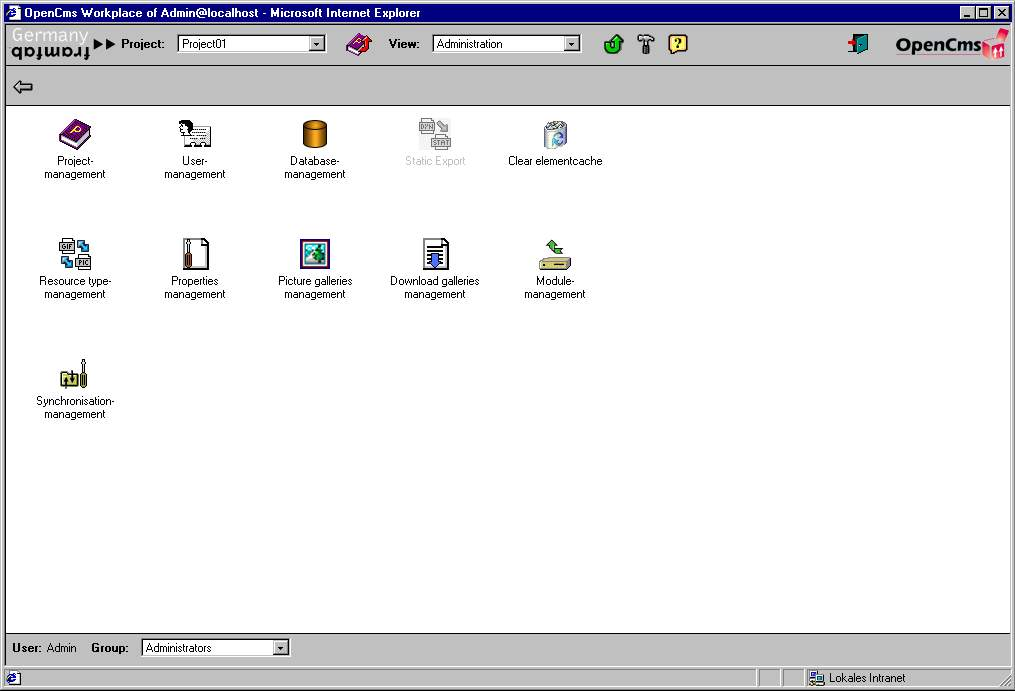
\includegraphics[width=\sgw]
                   {pics/templateMech/admin_point}
\caption[Administration view]
           {Administration view}
\label{AdView}
\end{center}
\end{figure}

The administration of modules is done under the administration view(Figure~\ref{AdView}).
Change to the administration view and then choose the item {\name module}.
In the next screen a list with the modules that are already installed is shown. Existing
modules can be deleted, administrated or exported. In this view existing modules can also
be added to the system (upload a module) or new modules can be created.

\begin{figure}[hbt]
\begin{center}
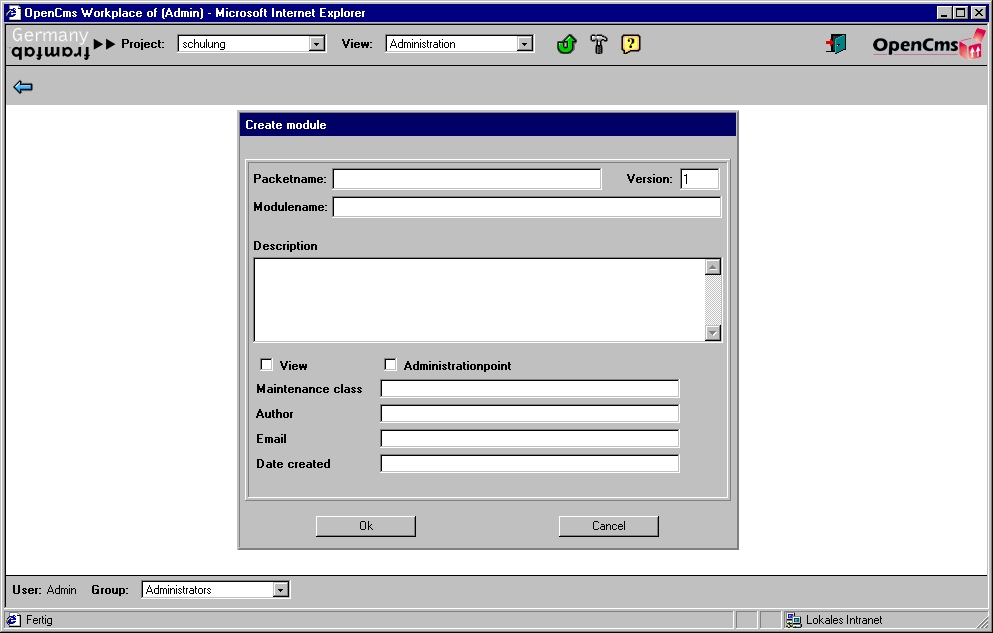
\includegraphics[width=\sgw]
                   {pics/templateMech/create_new}
\caption[Create a new module]
           {Create a new module}
\label{CreMod}
\end{center}
\end{figure}

The creation of a new module is done with the help of wizard (Figure~\ref{CreMod}).
Please notice that you have to
be within a project that contains the root-folder to be able to start the creation of module.
All necessary information can be inserted in input fields and most of them can easily be
changed later if wanted. Two names can be declarated. The first name determines the real name
of the module. It has to be a name that follows the java name conventions for package names.
For example, your module could be called {\name com.opencms.myModule}. This name has to be
determined at first and can�t be changed after the module was  created. Normally your module
contains
templates and Java classes as well. Please keep in mind that the name of your module and the
name of your java package in your development enviroment have to be exactly the same. Thus,
your classes for the above example should reside in the package {\name com.opencms.myModule}.
The other name that can be added is a "talking" name that describes the module. The item
{\name version} is the version number of the module as an integer. The checkbox {\name view}
has to be
choosen if the module should append a new view to openCms. The module can also provide a new
Administrationpoint. In this case the corresponding selectbox has to be choosen. Of course
your module don�t need to provide a new view in every case. You can specify a class that
handles events like deleting a module, uploading a module and changings of the parameters as
well.

\begin{figure}[hbt]
\begin{center}
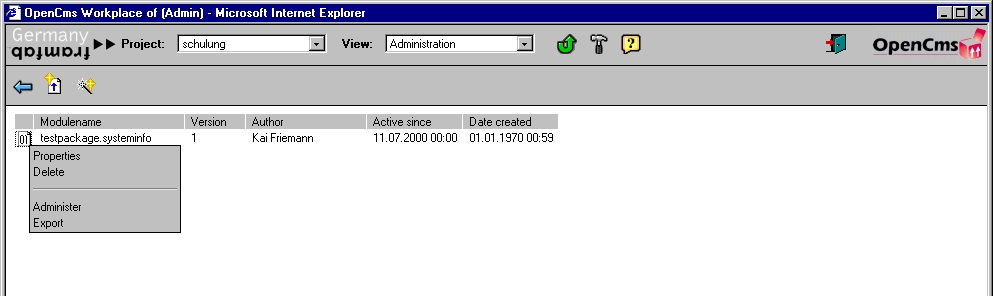
\includegraphics[width=\sgw]
                   {pics/templateMech/mod_list}
\caption[The list of modules]
           {The list of modules}
\label{ModList}
\end{center}
\end{figure}

Some more details can be determined after creating the module. Whe can specify certain
dependencies when choosing the item {\name administrate} from the context-sensitive menue of your
module.
It is possible that your module depends on several other  modules, that might have certain
version numbers. In this case these dependencies can be specified after the module has been
created (Figure~\ref{deps}).

\begin{figure}[hbt]
\begin{center}
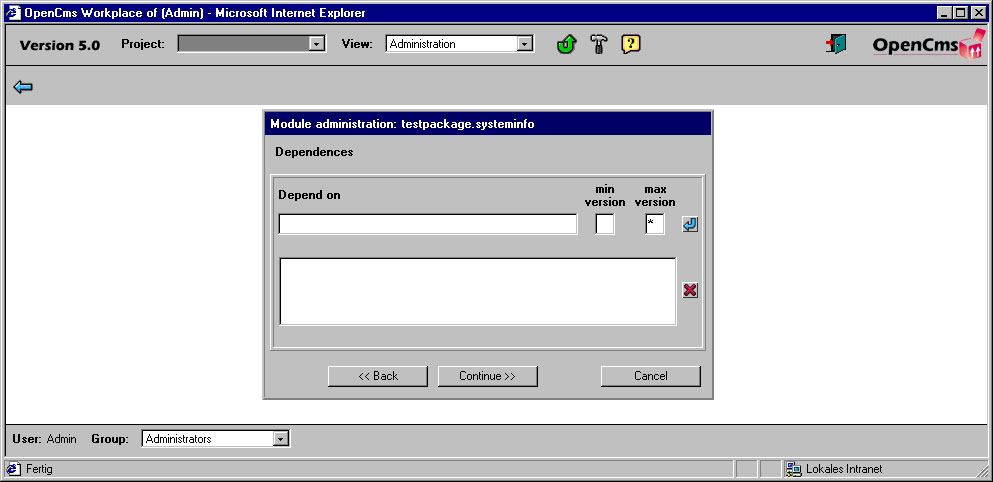
\includegraphics[width=\sgw]
                   {pics/templateMech/admin_2}
\caption[Dependencies to other modules]
           {Dependencies to other modules}
\label{deps}
\end{center}
\end{figure}

The  module mechanism uses  the module name to create certain directories. One important thing
when handling modules is to follow the recommended way of creating and storing files and folders.
The module mechanism creates some new folder-trees.
A directory {\dir package\_name} is created in the directory {\dir /moduledemos} for every new module.
In this directory should be a demoversion of your module. Normally this would be a body template
that makes usage of the mechanism you implemented. The entry point of your demo should always be
a file called {\name index.html}.
Another directory {\dir package\_name} is created within the {\dir /system/modules} directroy.
This dirctory
contains certain sub-dirctories that have been created by the module mechanism. A subdirectory
{\name administration} is created if you have choosen your module to provide a new administration
item in the administration view.

\subsubsection{Master templates}

All master templates that belong to your module have to be stored in the\\
{\dir /system/modules/package\_name/templates/} directory. You can choose the mastertemplate
from a
selectbox when you are creating a new page. Thus, OpenCms has to know where to look for them.
Other (sub-)templates that are used by your module should be stored inside another directory
within your module subtree. Only files that lie within your module subtrees can be found by
OpenCms when you export your module (what is the sense of every module).

\subsubsection{Classes that correspond to the Pages}

Your Java classes, i.e. the byte code, are also resources in the OpenCms system.
The module mechanism creates a further directory for these classes. For this reason, the name
of your module (e.g. com.opencms.examples.newsmodule) is splitted into subdirectories
(e.g. {\dir /com/opencms/examples/newsmodule/} ). You can use a JAR file, a zip file or class files.
While developing your module, you can leave the classes in your local file system within your
classpath. It is only important to upload the classes when you finish (and export) your module.
A mechanism to "synchronize" (or upload) the classes in an easy way will be discussed in part
~\ref{synchronisation}.

\subsubsection{Adding a new Administration Item}

When you change to the Administration view, a number of icons such as
{\name Project Administration} and
{\name User Administration} are displayed. This section describes how to add your own item. You
will need an icon in the form of a GIF file that fits in terms of size and style. If you would
like to have a variant for an inactive item, the file should have the same name with the
addition of {\name \_in} for inactive at the end of the file name, before the extension
{\name .gif.} Put
this image in the folder {\dir /system /modules/package\_name/pics/} and ensure that it's owner
and group are one of the three standard users and groups.
For every item that should be displayed, a new directory (for example {\name mymodule}) has to be
created in the {\dir /system /modules/package\_name/administration/} directory.
Then give the folder

{\dir /system /modules/package\_name/administration/mymodule/}

new properties by selecting 'Properties' from the context-sensitive menu:

\begin{table}\begin{center}
\begin{tabular}{|l|p{0.75\linewidth}|}
\hline
NavPos  &
This real number determines the order of the icons in the administration view. The
icons are ordered by increasing NavPos. To add your icon at the end select the highest of all
NavPos values in the other folders in the directory {\dir /system/workplace/administration/}.\\
NavText &
The tag for the subtitle of the icon in the language files you provide. You will
have to provide one or more language files with this subtitle in each language. The tag should
be the same in all language files.\\
Title  &
The name of the GIF file of the icon that is used in the Administration view
without the extension {\name .gif}.\\
\index{visiblemethod}  visiblemethod &
Visiblemethod is a method that returns a Boolean value. It returns true when the
icon is displayed to the current user in the current project. If it returns false, the icon is
not displayed. If you do not specify this method the icon will always be visible. You can enter
the name of the method here. When creating the new property you have to determine a method
(with its full path!) under the item {\name Enter Property value}. See folders in the
{\dir /system/workplace/administration/directory for an example}.\\
\index{activemethod} activemethod &
Activemethod is a method that returns a Boolean value. It returns true when
the icon is active, i.e. clickable. If false, the icon is still displayed but in an inactive
style, and without a link to the icon. If you do not specify this method the icon will always
be active. You can enter the name of the method here. When creating the new property you have
to determine a method (with its full path!) under the item {\name Enter Property value}. See folders
in the {\dir /system/workplace/administration/directory} for an example.\\
\hline
\end{tabular}
\caption[Properties] {Properties}
\label{direct}\end{center}
\end{table}


Here is an example for the properties:\\
\begin{xml}
NavPos = 7\\
NavText = mymodule.administration.icon.paybyclick\\
Title = paybyclick\\
visiblemethod = com.opencms.workplace.CmsWorkplaceDefault.isNotOnlineProject\\
\end{xml}

In the folder {\name mymodule}, create a page with the name index.html. This is the page that will be
displayed when the new item is click on.

You also have the ability to display several administration items when your item is clicked on,
as is currently done for the
{\name User Administration} and {\name Project Administration} items. Simply
add new subfolders in the\\
{\dir /system/modules/package\_name/administration/mymodule/} directory, give
them the same properties as above, an add icons and an index.html page to each subfolder. Please
notice that every directory that is created within the {\dir /administration/} directory will be
added as an administration item frome the module mechanism and an error will occur if you add
directories here that don�t follow these conventions.
In the Administration view there is an additional frame {\name admin\_head} for navigation just below
the toolbar. If you only want to use the standard frame with the blue back button then let this
frame be updated when your {\name index.html} is displayed by adding the following onLoad javascipt to
your body tag:{\code
<body onLoad="window.top.body.admin\_head.location.href='[path to the /system/workplace/action
folder]/administration\_head.html';"> }

Or create your own {\name admin\_head} frame. You might want to look at the picture or download
galleries that you can use as examples.

\subsubsection{Adding a new view}

It is also possible to add an entry in the view {\name selectbox}, similar to the entries for
{\name Explorer}, or {\name Administration}. If you have aktivated the checkbox
{\name view} when you created the
module, a directory with the name {\name view} has automatically been created within the
{\dir /system/modules/package\_name/} directory. In this case you have to put a file with the
name {\name index.html} into this directory. This is the html page that should be displayed when your
view has been selected from the selectbox. Of course there has to be a corresponding tag in
the language file.

\subsubsection{Language Files}
\index{Language Files}
OpenCms supports multiple languages on the workplace, and it is possible to run several
languages on the same server simultaneously. Users can select their preferred language by
clicking on the hammer icon and selecting the start settings. Currently, we only support German
and English but it is easy to write language files in another language by copying existing
files and translating them tag by tag. The developers welcome any suggestions and contributions
you may wish to make about language files. Please send your ideas to contributions@opencms.com.
To make multiple languages possible at all it is important that you put every piece of text that
appears on the workplace in the language file(s) of your module. This might seem long winded but
not doing this means that translating your module to another language will be very time and cost
intensive. Make sure to include the English version of your language file. The language files
are xml files that are stored in the folder {\dir /system/modules/package\_name/language/}.
This folder
contains subfolders for each supported language (de, uk). The language names correspont to their
top-level domain names. In each of these subfolders there is a language file
(e.g. {\name mymodule\_uk})
for the module. The name should be the same as that (packagename) of the module, say
com.opencms.mymodule, followed by an underscore and the language code.

Example:

Create an English language file
\begin{xml}
/system/modules/com.opencms.mymodule/language/uk/com.opencms.mymodule\_uk
\end{xml}


that looks like this:
\begin{xml}
<?xml version="1.0"?>\\
<LANGUAGE>\\
\xtaba   <name>English</name>\\
\xtaba   <com\_opencms\_mymodule>\\
\xtabb     <!-- fill in your tags here -->\\
\xtaba   </com\_opencms\_mymodule>\\
</LANGUAGE>\\
\end{xml}


Make sure to include your module name at the top level because all of the language files that
belong to the same language are merged, and doing this avoids file collisions. Within the
language file, dots (".") have to be replaced with underscores ("\_").

\subsubsection{Documentation}
\index{Documentation}
Modules should be well documented. The module mechanism creates two folders.
The directory {\dir system/modules/package\_name/doc} is created to hold some textual
documentation. A file {\name index.html} should be placed here.
The directory {\dir moduledemos/package\_name} is automatically created as well. Inside this
directroy has to be a demo of the module.
The demo is a template, that uses all features of the module in
a simple way.
If you create a new page within this demo directoy, the corresponding content file is created
inside the {\dir /content/bodys} directory.
Thes files are as well found when exporting the module.

\subsubsection{Directories}

Here is a short overview of the directories that are created by the module mechanism:

\begin{xml}
/moduledemos/com.opencms.mymodule\\
/system/modules/com.opencms.mymodule/\\
\xtaba                    /administration \\
\xtabb                         /view \\
\xtabb                         /templates \\
\xtabb                         /language \\
\xtabc                         /de \\
\xtabc                                 /uk\\
\xtabb                            /doc\\
/system/classes/com/opencms/mymodule\\
\end{xml}

\section{Stylesheets}
%============================================================================
\index{Stylesheets}

Stylesheets can be used in OpenCms just like in standard html. There is only one
point concerning Stylesheets which is worth to be mentioned here in the documentation.
This is that stylesheet information can be used in the WYSIWYG-Editor as well.
This way WYSIWYG-behaviour can be realized even when using stylesheets.
There is only one change within the mastertemplate necessary to achieve this
behaviour. The special tag {\name stylesheet} has to be inserted and the path to the
stylesheet-file has to be determined.
Here is an example of a mastertemplate which includes Stylesheet information and allows
the WYSIWYG-Editor to use them as well.

\begin{xml}
<?xml version="1.0"?>\\
<XMLTEMPLATE>\\
<stylesheet>system/modules/.../css/style.css</stylesheet>\\

<TEMPLATE>\\
<![CDATA[\\
<html>\\
<head>\\
\xtaba  <title>]]><method name="getTitle"/><![CDATA[</title>\\
\xtaba  <meta http-equiv="Content-Type" content="text/html;\\
\xtabb      charset=iso-8859-1">\\
\xtaba  <link rel="stylesheet" href="]]><method\\
\xtabb      name="getServletPath"/>\\
\xtabb      <![CDATA[system/modules/.../css/style.css">\\
</head>\\

<body ...\\
\end{xml}

As you can see, the file {\name style.css} is referenced twice.
The first reference is inside the {\name stylesheet}-tag. This is the specification
which makes the stylesheet information useable within the WYSIWYG-Editor.
The second reference is just one normal way a stylesheet file can be used in html.
This specification makes the stylesheet information useable in the html-page.



%%% Local Variables:
%%% mode: latex
%%% TeX-master: "OpenCmsDoc"
%%% End:
